\documentclass[sigconf]{acmart}

\fancyhf{} % Remove fancy page headers 
% \fancyhead[C]{Anonymous submission \#9999 to ACM CCS 2017} % TODO: replace 9999 with your paper number
\fancyfoot[C]{\thepage}

\setcopyright{none} % No copyright notice required for submissions
% \acmConference[Anonymous Submission to ACM CCS 2017]{ACM Conference on Computer and Communications Security}{Due 19 May 2017}{Dallas, Texas}
% \acmYear{2017}

\settopmatter{printacmref=false, printccs=true, printfolios=true} % We want page numbers on submissions

%%\ccsPaper{9999} % TODO: replace with your paper number once obtained

%packages
\usepackage{natbib}
\usepackage{amsmath}
\usepackage{amsthm}
\usepackage{mathtools}
\usepackage{mdframed}
\usepackage{subfigure}
\usepackage{booktabs}
% \usepackage{hyperref}
\usepackage{subfigure}
\usepackage{siunitx} % Provides the \SI{}{} and \si{} command for typesetting SI units
\usepackage{graphicx} % Required for the inclusion of images
% \usepackage{natbib} % Required to change bibliography style to APA
\usepackage{datetime}
\usepackage{lscape}
\usepackage{algorithm}
\usepackage{algorithmic}
\usepackage{xspace}
\usepackage[english]{babel} % English language/hyphenation
\usepackage{proof}
\usepackage{booktabs} % Top and bottom rules for tables
\usepackage[colorlinks, allcolors = blue,]{hyperref}
\usepackage{accents}
\usepackage{amsfonts}
\usepackage{stmaryrd}
\usepackage{amsmath,amsthm,amssymb,latexsym} 
\usepackage{microtype}
\usepackage{graphicx}
\usepackage{subfigure}
\usepackage{booktabs} % for professional tables
\usepackage{hyperref}
\usepackage{icml2019}
\usepackage{lipsum}

\usepackage{authblk}


%new commands
\newcommand{\theHalgorithm}{\arabic{algorithm}}
\newtheorem{definition}{Definition}
\usepackage{cancel}
\usepackage[normalem]{ulem}
\newcommand{\dataobs}{\textbf{x}}
\newcommand{\adj}[2]{\textbf{adj}(#1,#2)}
\newcommand{\candidateset}{\mathcal{R}_{\textup{post}}}
\newcommand{\bprior}{\boldsymbol{\beta}_{\textup{prior}}}
\newcommand{\bysinfer}{\mathsf{Infer}}
\newcommand{\betad}{\mathsf{Beta}}
\newcommand{\betaf}{\textup{B}}
\newcommand{\mbetaf}{\boldsymbol{\textup{B}}}
\newcommand{\vtheta}{\boldsymbol{\theta}}
\newcommand{\valpha}{\boldsymbol{\alpha}}
\newcommand{\vbeta}{\boldsymbol{\beta}}
\newcommand{\lapmech}{\mathsf{LSDim}}
\newcommand{\ilapmech}{\mathsf{LSHist}}
\newcommand{\binomial}[2]{\mathsf{Bin}(#1, #2)}
\newcommand{\multinomial}[2]{\mathsf{Mult}(#1, #2)}
\newcommand{\expmech}{\mathsf{EHD}}
\newcommand{\hexpmech}{\mathsf{EHDS}}
\newcommand{\lexpmech}{\mathsf{EHDL}}
\newcommand{\hexpmechd}{\mathsf{expMech}^{D}_{\hellinger}}
\newcommand{\privinfer}{\mathsf{PrivInfer}}
\newcommand{\hlg}{\mathsf{H}}
\newcommand{\dirichlet}[1]{\mathsf{Dir}(#1)}
\newcommand{\alphas}{\boldsymbol{\alpha}}
\newcommand{\xis}{\boldsymbol{\xi}}
\newcommand{\iverson}[1]{[#1]}
\newcommand{\datauni}{\mathcal{X}}
\newcommand{\hellinger}{\mathcal{H}}
\newcommand{\ux}[1]{u(\textbf{x}, {#1})}
\newcommand{\uxadj}[1]{u(\textbf{x}', {#1})}
\newcommand{\cardinality}[2]{\mathcal{C}^{#1}_{#2}}
\newcommand{\range}{\mathcal{O}}
\newcommand{\nomalizer}[1]{\sum\limits_{r'\in \mathcal{R}_{\textup{post}}} \exp \big(\frac{-\epsilon\cdot \mathcal{H} (\mathsf{BI}(#1),r')}{4 \cdot S(#1)}\big)}

\newcommand{\unomalizer}[1]{\sum\limits_{r'\in \mathcal{R}_{\textup{post}}} \exp \big(\frac{-\epsilon\cdot u(#1, r')}{4 \cdot S(#1)}\big)}


\newcommand{\hexpmechPr}[2]{\underset{z \thicksim \hexpmech(#1)}{\Pr}\left[ #2 \right]}
\newcommand{\lapmechPr}[2]{\underset{z \thicksim \lapmech(#1)}{\Pr}\left[ #2 \right]}

\newcommand{\ilapmechPr}[2]{\underset{
{z \thicksim \ilapmech(#1)}
}{\Pr}\left[ #2 \right]}

\newtheorem{thm}{Theorem}[section]

\newtheorem{lem}{Lemma}[section]

\newtheorem{assert}{Assertion}[lem]
\newcommand{\lap}[2]{\mathsf{Lap}(#1, #2)}
\newcommand{\todo}[1]{{\footnotesize \color{red}\textbf{[[ #1 ]]}}}
\usepackage{accents}



\begin{document}
\title{Tailoring Differentially Private Bayesian Inference to Distance Between Distributions}
\subtitle{Extended Abstract}


\author{Mark Bun}
\affiliation{%
  \institution{Princeton University}
}
\email{mbun@cs.princeton.edu}

\author{Gian Pietro Farina}
\affiliation{%
  \institution{University at Buffalo, SUNY}
}
\email{gianpiet@buffalo.edu}


\author{Marco Gaboardi}
\affiliation{%
  \institution{University at Buffalo, SUNY}
}
\email{gaboardi@buffalo.edu}

\author{Jiawen Liu}
\affiliation{%
  \institution{University at Buffalo, SUNY}
}
\email{jliu223@buffalo.edu}

\begin{abstract} Bayesian inference is a statistical method which
allows one to derive a \emph{posterior} distribution over a parameter,
starting from a \emph{prior} distribution and observed data. Settings
where sensitive individual information is involved, different
approaches have been taken to make this process differentially
private. \citet{dimitrakakis2014robust}, and \citet{wang2015privacy},
for instance, proved that, under specific conditions, sampling from
the posterior distribution is already differentially private. Other
works, e.g., \cite{zhang2016differential}, \cite{foulds2016theory},
designed differentially private mechanisms that output a
representation of the full posterior distribution. Also, accuracy of
these mechanisms was measured using metrics on the space of the
numeric parameters of the posterior distribution, e.g., the
$\ell_1$-norm.

In this work we present a new differentially private algorithm to
compute the posterior in a Beta-Binomial system and in a
Dirichlet-Multinomial system. We apply the exponential mechanism to
the smooth sensitivity of a metric on probability distributions; we
measured the accuracy of the process by using the same metric. We
compared the accuracy of this approach with the ones based on
$\ell_1$-norm. Experimental results show that when the data size is
small or when the parameters of the prior distribution are large, the
former outperforms the latter.

\end{abstract}


% TODO: replace this section with code generated by the tool at https://dl.acm.org/ccs.cfm
% \begin{CCSXML}
% <ccs2012>
% <concept>
% <concept_id>10002978.10003029.10011703</concept_id>
% <concept_desc>Security and privacy~Usability in security and privacy</concept_desc>
% <concept_significance>500</concept_significance>
% </concept>
% </ccs2012>
% \end{CCSXML}

% \ccsdesc{Security and privacy~Use https://dl.acm.org/ccs.cfm to generate actual concepts section for your paper}
% % -- end of section to replace with generated code

\keywords{Differential privacy, Bayesian inference, Hellinger distance} % TODO: replace with your keywords

\maketitle

\section{An informal motivation}
\label{sec_intro}
Publishing the posterior distribution inferred from a sensitive dataset can
leak information about individuals on the dataset.
Hence, in order to protect the dataset, random noise is added to the posterior belief before releasing it.
The amount of the noise that must be introduced
depends on the privacy parameter $\epsilon$ and the sensitivity of the inference to
small changes in the data set. 
Sensitivity can be computed in many different ways based on which metric space
is imposed on the output set of the mechanism. In the literature on private Bayesian
inference (\cite{zhang2016differential,xiao2012bayesian}), it is only measured with
respect to the vector of numbers parametrizing the output distribution using, e.g. the $\ell_1$ norm.
A more natural approach which we explore here, is to measure sensitivity with respect to a metric on the space of inferred probability distributions.
A re-loved question is that of how to measure accuracy. Again,
this can be answered in different ways based on the metric imposed on the output space, and yet again
only in few works in literature (e.g. \cite{zhang2016differential})
distances between probability measures have been used for these purposes.


The question that this work aims at answering is whether
an approach based on probability metrics can improve on the accuracy of approaches based on metrics over
the numeric parameters of the distributions. 
We will see that in some cases this can happen.


\section{Bayesian Inference Background}
\label{sec_background}
Given a prior belief $\Pr(\theta)$ on some parameter $\theta$,
and an observation $\dataobs$, the posterior distribution on $\theta$ given $\dataobs$ is computed as:
\[
  \Pr(\theta | \dataobs) = \frac{\Pr(\dataobs | \theta) \cdot \Pr(\theta)}{\Pr(\dataobs)}
\]
where the expression $\Pr(\dataobs | \theta)$ denotes the
\emph{likelihood} of observing $\dataobs$ under a value of
$\theta$. Since we consider $\dataobs$ to be fixed, the likelihood is
a function of $\theta$.
For the same reason $\Pr(\dataobs)$ is a constant independent of $\theta$.
Usually in statistics the prior distribution $\Pr(\theta)$ is chosen so that it represents
the initial belief on $\theta$, that is, when no data has been observed. In practice though,
prior distributions and likelihood functions are usually chosen so that the posterior
belongs to the same \emph{family} of distributions. In this case we say that the prior
is conjugate to the likelihood function. Use of a conjugate prior
simplifies calculations and allows for inference to be performed in a
recursive fashion over the data.
In this work we will consider a specific instance of Bayesian inference and one of its generalizations.
Specifically, we will consider the situation where $\theta$ represents
the parameter --informally called \emph{bias}-- of a Bernoulli
distributed random variable, and its immediate generalization where
the parameter $\vtheta$ represents the vector of parameters of a
categorically distributed random variable.  In the former case, the
prior distribution over $\theta\in [0,1]$ is going to be a beta
distribution, $\betad(\alpha, \beta)$, with parameters
$\alpha,\beta\in\mathbb{R}^{+}$, and with p.d.f:

\[
  \Pr(\theta)\equiv \frac{\theta^{\alpha} (1- \theta)^{\beta}}{\betaf(\alpha,\beta)}
\]
where $\betaf(\cdot,\cdot)$ is the beta function.
The data $\dataobs$ will be a sequence of $n\in\mathbb{N}$ binary values, that is $\dataobs= (x_1,\dots x_n), x_i\in\{0,1\}$, and the likelihood function is:
\[
  \Pr(\dataobs | \theta)\equiv \theta^{\Delta \alpha}(1-\theta)^{n - \Delta \alpha}
\]
where $\Delta \alpha = \displaystyle\sum_{i=1}^{n}x_i$.
From this it can easily be derived that the posterior distribution is:
\[
  \Pr(\theta|\dataobs)=\betad(\alpha + \Delta \alpha,\beta + n - \Delta \alpha)
\]
In the latter case the prior distribution over $\vtheta\in [0,1]^{k}$
is given by a Dirichelet distribution, $\dirichlet(\valpha)$, for $k\in\mathbb{N}$,
and $\valpha\in(\mathbb{R}^{+})^{k}$, with p.d.f:
\[
  \Pr(\vtheta)\equiv\frac{1}{\mbetaf(\valpha)}\cdot \displaystyle\prod_{i=1}^{k}{\theta_i^{\alpha_i-1}}
\]
where $\mbetaf(\cdot)$ is the generalized beta function.
The data $\dataobs$ will be a sequence of $n\in\mathbb{N}$ values
coming from a universe $\datauni$, such that $\mid\datauni \mid=k$.
The likelihood function will be:
\[
  \Pr(\dataobs|\vtheta)\equiv \displaystyle\prod_{a_i\in\datauni}\theta_{i}^{\Delta \alpha_i},
\]
with $\Delta \alpha_i=\displaystyle\sum_{j=1}^{n}\iverson{x_j=a_i}$, where $\iverson{\cdot}$ represents Iverson bracket notation.
Denoting by $\Delta\valpha$ the vector $(\Delta\alpha_1,\dots \Delta\alpha_k)$ the posterior distribution over $\vtheta$ turns out to be
\[
  \Pr(\vtheta|\dataobs)=\dirichlet(\valpha+\Delta \valpha). 
\]
where $+$ denotes the componentwise sum of vectors of reals. 


\section{The Problem and Baseline approach}
\label{sec:base}
We are interested in designing a mechanism for privately releasing the full posterior
distributions derived in section \ref{sec_background}, as opposed to just sampling from them.
It's worth noticing that the posterior distributions are fully characterized
by their parameters, and the family (beta, Dirichlet) they belong to. Hence, in case of the
Beta-Binomial model we are interested in releasing a private version of the pair of
parameters $(\alpha',\beta')=(\alpha + \Delta \alpha,\beta + n - \Delta \alpha)$, and
in the case of the Dirichlet-Multinomial model we are interested in a private version of
$\valpha'=(\valpha + \Delta \valpha)$. \citet{zhang2016differential} and \citet{xiao2012bayesian}
have already attacked this problem by adding independent Laplacian noise to the
parameters of the posteriors. That is, in the case of the Beta-Binomial system,
the value released would  be: $(\tilde\alpha,\tilde\beta)=(\alpha +  \widetilde{\Delta \alpha},\beta + n - \widetilde{\Delta \alpha})$
where $\widetilde{\Delta \alpha}\sim Lap(\Delta \alpha, \frac{2}{\epsilon})$,
and where $Lap(\mu,\nu)$ denotes a Laplace random variable with mean $\mu$ and scale $\nu$.
This mechanism is $\epsilon$-differentially private, and the noise is
calibrated w.r.t. to a sensitivity of 2 which is derived by using
$\ell_1$ norm over the pair of parameters. Indeed, considering two
adjacent\footnote{Given $\dataobs, \dataobs'$  we say that $\dataobs$ and $\dataobs'$ are adjacent and we write, $\adj{\dataobs}{\dataobs'}$, iff\\
$\displaystyle \sum_{i}^{n}\iverson{x_i = x'_i }\leq 1$. } data observations
$\dataobs, \dataobs'$, that, from a unique prior, give rise to two posterior
distributions, characterized by the pairs
$(\alpha',\beta')$ and $(\alpha'',\beta'')$ then
$|\alpha'-\alpha''|+|\beta'-\beta''|\leq 2$.
This argument extends similarly to the Dirichelet-Multinomial system.

\noindent Also, in previous works, the accuracy of the posterior was measured again with respect to $\ell_1$ norm. That is, an upper bound was given on
\[
  \Pr[|\alpha - \tilde\alpha| + |\beta - \tilde\beta |\geq \gamma ]
\]
where $(\alpha, \beta), (\tilde\alpha,\tilde\beta)$ are as  defined above.
In this work we will use a metric based on a different norm to compute the sensitivity
and provide guarantees on the accuracy. In particular we will consider a metric
over probability measures and not over the parameters that represent them.
Specifically, we will use the Hellinger distance $\hellinger(\cdot,\cdot)$.
Our choice to use Hellinger distance is motivated by two facts, first of all it simplifies
calculations in the case of the probabilistic models considered here
and second of all it also automatically yields bounds on the total variation distance, which represents also the maximum advantage
an unbounded adversary can have in distingishing two distributions. 
Given two beta distributions
$\boldsymbol{\beta}_1=\betad(\alpha_1, \beta_1),$ and $\boldsymbol{\beta}_2=\betad(\alpha_2, \beta_2)$ the following equality holds 
\[
  \hellinger(\boldsymbol{\beta}_1, \boldsymbol{\beta}_2)=
  \sqrt{1 - \frac{\betaf(\frac{\alpha_1 + \alpha_2}{2}, \frac{\beta_1 + \beta_2}{2})}{\sqrt{\betaf(\alpha_1,\beta_1)\betaf(\alpha_2,\beta_2)}}}
\]
The same change of metric will be applied to the experimental accuracy guarantees.
% \section{Technical Problem Statement}
% \label{sec_bayesInfer}
% The posterior belief about parameters $\xis$ is inferred from the
% group of sensitive data. Because it is usually published in form of a
% distribution, for example, $\betad(\alpha',\beta'), \cdots,$ itself
% can relieve a lot of information about sensitive data. So, the
% sensitive information we want to protect here is the posterior belief,
% i.e., $Pr(\xis | \dataobs)$, rather than just a sample drew from
% it\cite{foulds2016theory}. Then it will be better if we can use a
% distance over two distributions to measure the accuracy than a
% distance over just parameters or values when we are protecting a
% distribution, for instance, Hellinger distance in our paper. When we
% measure the accuracy between true posterior and protected posterior
% using Hellinger distance, it would be better we can have a protection
% mechanism based on Hellinger distance. However, current mechanisms are
% mainly based on $l_1$ norm by Laplace mechanism
% \cite{zhang2016differential} \cite{xiao2012bayesian}. That's why we
% design our exponential mechanism over Hellinger distance to protect
% the whole posterior distribution.


% \section{Baseline Approach - Laplace Mechanism}
% \label{sec_lap}
% Our baseline approach come from the algorithm designed by \citet{zhang2016differential} that adding Laplace noise (\citet{dwork2014algorithmic}) to posterior parameters to preserve privacy. They perturbed the parameter updates of $\betad$ distribution from Bayesian inference and truncated to rule out invalid $\betad$ parameters to get the protected posteriors.
% Furthermore, we extend their algorithm to the case of $m$ dimensional Dirichlet distributions, where we add $(m-1)$ i.i.d. Laplace noises $\{Lap_1 , Lap_2, \cdots, Lap_{m-1} \}$ and truncate in the same way. 
% %where $Lap_i = floor(Y)$, $Y \sim Lap(\frac{2}{\epsilon})$. 
% The private posterior is $\dirichlet(\valpha + \Delta \valpha')$, where $\Delta \valpha'$ is the perturbed parameter updates.

\section{Our Approach - Exponential Mechanism with Smooth Sensitivity}
\label{sec_smoo}
Given a prior distribution $\bprior=\betad(\alpha, \beta)$ and a sequence of $n$ observations $\dataobs\in\{0,1\}^n$, we define the follwing set:

\[
  \betaset\equiv\{\betad(\alpha',\beta')\mid \alpha'=\alpha+\Delta\alpha, \beta'=\beta+n-\Delta\alpha\}
\]

where $\Delta\alpha$ is as defined in Section
\ref{sec_background}. Notice that $\betaset$ has $n + 1$ elements, and
the Bayesian Inference process will produce an element from $\betaset$
that we denote by $\bysinfer(\dataobs)$ -- we don't explicitely
parametrize the result by the prior, which from now on we consider
fixed and we denote it by $\bprior$.


We can now define the mechanism $\hexpmech$ which, given in input a
sequence of observations $\dataobs$ and parameters $\epsilon>0$ and
$\delta>0$, produces an element $r$ in $\betaset$ with probability:

\begin{equation*}
\underset{z \thicksim \hexpmech}{\Pr}[z=r] = \frac {exp\big(\frac{-\epsilon\cdot\hellinger(\bysinfer(\dataobs),r)}{2\cdot S(\dataobs)}\big)}
{\displaystyle\sum_{r\in\betaset} exp\Big(\frac{-\epsilon\cdot\hellinger(\bysinfer(\dataobs),r)}{2\cdot S(\dataobs)}\Big)}.
\end{equation*}

This mechanism is based on the basic exponential mechanism
\cite{talwar}, with $\betaset$ as the range and
$\hellinger(\cdot,\cdot)$ as the scoring function. The difference is
that in this mechanism we don't calibrate the noise w.r.t. to the
global sensitivity of the scoring function but w.r.t. to the smooth
sensitivity $S(\dataobs)$ -- defined by \citet{nissim2007smooth}-- of
$\hellinger(\bysinfer(\dataobs), \cdot)$. The smooth sensitivity is
computed as follows:
\begin{equation}
  \label{eq:smooth}
   S(\dataobs)=\max_{\dataobs' \neq \dataobs, \dataobs' \in \{0,1\}^{n}}\bigg \{\Delta_{l}\bigg (\hellinger(\bysinfer(\dataobs'),\cdot)\bigg )\cdot e^{-\gamma\cdot d(\dataobs, \dataobs')}\bigg\},
\end{equation}
where $d$ is the Hamming distance between two datasets, $\gamma =
\gamma(\epsilon, \delta)$ is a function of $\epsilon$ and $\delta$ to
be determined later, and where $\Delta_{l}\bigg
(\hellinger(\bysinfer(\dataobs'),\cdot)\bigg )$ denotes the local
sensitivity at $\bysinfer(\dataobs')$, or equivalently at $\dataobs'$,
of the scoring function used in our mechanism. That is:
\begin{equation*}
\Delta_{l}\bigg (\hellinger(\bysinfer(\dataobs'),\cdot)\bigg )=\max_{\dataobs'' \in \datauni^n:\adj{\dataobs'}{\dataobs''}, r\in \betaset}\lvert \hellinger(\bysinfer(\dataobs'), r) - \hellinger(\bysinfer(\dataobs''), r)\rvert.
\end{equation*}

This mechanism also extends to the Dirichlet-Multinomial system $\dirichlet(\valpha)$ by rewriting the Hellinger distance as:
\[
  \hellinger(\dirichlet(\valpha_1), \dirichlet(\valpha_2)) = \sqrt{1 - \frac{\betaf(\frac{\valpha_1 + \valpha_2}{2})}{\sqrt{\betaf(\valpha_1) \betaf(\valpha_2)}}},
\]
and by replacing the $\betaset$ with set of posterior Dirichlet
distributions candidates. Also, the smooth sensitivity $S(\dataobs)$
in (\ref{eq:smooth}) will be computed by letting $\dataobs'$ range
over all the elements in $\datauni^{n}$ adjacent to $\dataobs$. Notice
that $\betaset$ has $\binom{n + 1}{m - 1}$ elements in this case. We
will denote by $\hexpmechd$ the mechanism for the
Dirichlet-Multinomial system.
% In what follows, we will use a correspondence between the probability
%  $\underset{z \thicksim \hexpmech(x)}{Pr}[z = r]$ of every
%  $r\in\betaset$ and the probability 
%  $\underset{z \thicksim \hexpmech(x)}{Pr}[\hlg(\bysinfer(x),z) =
%  \hlg(\bysinfer(x),r)]$ for the utility score for $r$. In particular, for every
%  $r\in\betaset$ we have:
% $$
% \underset{z \thicksim \hexpmech(x)}{Pr}[z = r]=
% \frac{1}{2}\Big (\underset{z \thicksim \hexpmech(x)}{Pr}[\hlg(\bysinfer(x),z) =
%  \hlg(\bysinfer(x),r)]\Big )
% $$
% To see this, it is enough to notice that: $\underset{z \thicksim \hexpmech(x)}{Pr}[z = r]$ is proportional too $\hlg(\bysinfer(x),r)$, i.e., $u(x,z)$. We can derive, if $u(r,x) = u(r',x)$ then $\underset{z \thicksim \hexpmech(x)}{Pr}[z = r] = \underset{z \thicksim \hexpmech(x)}{Pr}[z = r']$. We assume the number of candidates $z \in \mathcal{R}$ that satisfy $u(z,x) = u(r,x)$ is $|r|$, we have  $\underset{z \thicksim \hexpmech(x)}{Pr}[u(z,x) = u(r,x)] = |r| \underset{z \thicksim \hexpmech(x)}{Pr}[z = r]$. Because Hellinger distance  $\hlg(\bysinfer(x),z)$ is axial symmetry, where the $\bysinfer(x)$ is the symmetry axis. It can be infer that $|z| = 2$ for any candidates, apart from the true output, i.e., $\underset{z \thicksim \hexpmech(x)}{Pr}[u(z,x) = u(r,x)] = 2 \underset{z \thicksim \hexpmech(x)}{Pr}[z = r]$. This parameter can be eliminate in both sides in proof.

% In our private Bayesian inference mechanism, we set the $\beta$ as $\ln(1 - \frac{\epsilon}{2 \ln (\frac{\delta}{2 (n + 1)})})$. 
The following result guarantees that the mechanisms are indeed differentially private.

\begin{theorem}[Privacy] 
\label{thm:privacy}
  For  $\gamma=\ln(1 - \frac{\epsilon}{2 \ln (\frac{\delta}{2 (n + 1)})})$, both
  $\hexpmech$ and $\hexpmechd$ are $(\epsilon,\delta)$-differentially private.
\end{theorem}




% \subsection{Sliding Property of Exponential Mechanism}
% \begin{lem}
% Consider the exponential mechanism  $\sexpmech(x,u,\mathcal{R})$
% calibrated on the smooth sensitivity. Let $\lambda = f(\epsilon,
% \delta)$, $\epsilon\geq 0$ and $|\delta| < 1$. Then, the following \emph{sliding property} holds:
% \begin{equation*}
% \underset{r \thicksim \hexpmech(x)}{Pr}[u(r,x) = \hat{s}]
% \leq
% e^{\frac{\epsilon}{2}} \underset{r \thicksim \hexpmech(x)}{Pr}[u(r,x) = (\Delta + \hat{s})] + \frac{\delta}{2},
% \end{equation*}

% \end{lem}

% \begin{proof}

% We denote the normalizer of the probability mass in $\hexpmech(x)$: $\sum_{r' \in \mathcal{R}}exp(\frac{\epsilon u(r',x)}{2 S(x)})$ as $NL(x)$:
% \begin{equation*}
% \begin{split}
% LHS 
%   = \underset{r \thicksim \hexpmech(x)}{Pr}[u(r,x) = \hat{s}]
% & = \frac{exp(\frac{\epsilon \hat{s}}{2 S(x)})}{NL(x)}\\
% & = \frac{exp(\frac{\epsilon (\hat{s} + \Delta - \Delta)}{2 S(x)})}{NL(x)}\\
% & = \frac{exp(\frac{\epsilon (\hat{s} + \Delta)}{2 S(x)} + \frac{- \epsilon \Delta}{2 S(x)})}{NL(x)}\\
% & = \frac{exp(\frac{\epsilon (\hat{s} + \Delta)}{2 S(x)})}{NL(x)} \cdot e^{\frac{- \epsilon \Delta}{2 S(x)})}.\\
% \end{split}
% \end{equation*}

% By bounding the $\Delta \geq -S(x)$, we can get:

% \begin{equation*}
% \begin{split}
% \frac{exp(\frac{\epsilon (\hat{s} + \Delta)}{2 S(x)})}{NL(x)} \cdot e^{\frac{- \epsilon \Delta}{2 S(x)}}
% & \leq \frac{exp(\frac{\epsilon (\hat{s} + \Delta)}{2 S(x)})}{NL(x)} \cdot e^{\frac{\epsilon}{2}}\\
% &  =  e^{\frac{\epsilon}{2}} \underset{z \thicksim \hexpmech(x)}{Pr}[u(r,x) = (\Delta + \hat{s})] \leq RHS\\
% \end{split}
% \end{equation*}

% \end{proof}

% \subsection{Dilation Property of Exponential Mechanism}
% \begin{lem}
% for any exponential mechanism $\hexpmech(x)$, $\lambda < |\beta|$, $\epsilon$, $|\delta| < 1$ and $\beta \leq \ln(1 - \frac{\epsilon}{2 \ln (\frac{\delta}{2 (n + 1)})})$, the dilation property holds:

% \begin{equation*}
% \underset{z \thicksim \hexpmech(x)}{Pr}[u(z,x) = c]
% \leq
% e^{\frac{\epsilon}{2}} \underset{z \thicksim \hexpmech(x)}{Pr}[u(z,x) = e^{\lambda} c] + \frac{\delta}{2},
% \end{equation*}
% where the sensitivity in mechanism is still smooth sensitivity as above.
% \end{lem}

% \begin{proof}

% The sensitivity is always greater than 0, and our utility function $-\hlg(\bysinfer(x),z)$ is smaller than zero, i.e., $u(z,x) \leq 0$, we need to consider two cases where $\lambda < 0$, and $\lambda > 0$:

% We set the $h(c) = Pr[u(\hexpmech(x)) = c] = 2\frac{exp(\frac{\epsilon z}{2 S(x)})}{NL(x)}$.

% We first consider $\lambda < 0$. In this case, $1 < e ^ {\lambda}$, so the ratio $\frac{h(c)}{h(e^{\lambda}c)} = \frac{exp(\frac{\epsilon c}{2 S(x)})}{exp(\frac{\epsilon (c \cdot e^{\lambda})}{2 S(x)})}$ is at most $\frac{\epsilon}{2}$.

% Next, we proof the dilation property for $\lambda > 0$, The ratio of $\frac{h(c)}{h(e^{\lambda}c)}$ is $\exp(\frac{\epsilon}{2} \cdot \frac{u(\hexpmech(x)) (1 - e^{\lambda})}{S(x)})$. Consider the event $G = \{ \hexpmech(x) : u(\hexpmech(x)) \leq \frac{S(x)}{(1 - e^{\lambda})}\}$. Under this event, the log-ratio above is at most $\frac{\epsilon}{2}$. The probability of $G$ under density $h(c)$ is $1 - \frac{\delta}{2}$. Thus, the probability of a given event $z$ is at most $Pr[c \cap G] + Pr[\overline{G}] \leq e^{\frac{\epsilon}{2}} Pr[e^{\lambda}c \cap G] + \frac{\delta}{2} \leq e^{\frac{\epsilon}{2}} Pr[e^{\lambda}c] + \frac{\delta}{2}$.\\


% \textbf{Detail proof:}
% \begin{itemize}

%   \item $\lambda < 0$

%     The left hand side will always be smaller than 0 and the right hand side greater than 0. This will always holds, i.e.
%     \begin{equation*}
%     \end{equation*}
%   \item $\lambda > 0$


% Because $\hat{s} = u(r)$ where $r \thicksim \hexpmech(x)$, we can substitute $\hat{s}$ with $u(\hexpmech(x))$. Then, what we need to proof under the case $\lambda > 0$ is:
% \begin{equation*}
% u(\hexpmech(x)) \leq \frac{S(x)}{(1 - e ^ {\lambda})}
% \end{equation*}
% By applying the accuracy property of exponential mechanism, we bound the probability that the equation holds with probability:
% \begin{equation*}
% \begin{split}
% Pr[u(\hexpmech(x)) \leq \frac{S(x)}{(1 - e ^ {\lambda})}] 
% & \leq \frac{|\mathcal{R}|exp(\frac{\epsilon S(x)}{(1 - e ^ {\lambda})}/2 S(x))}{|\mathcal{R}_{OPT}| exp(\epsilon OPT_{u(x)}/2 S(x))}\\
% \end{split}
% \end{equation*}

% In our Bayesian Inference mechanism, the size of the candidate set $\mathcal{R}$ is equal to the size of observed data set plus 1, i.e., $n + 1$, and $OPT_{u(x)} = 0$, then we have:
% \begin{equation*}
% \begin{split}
% Pr[u(\hexpmech(x)) \leq \frac{S(x)}{(1 - e ^ {\lambda})}] 
% & = (n + 1)exp(\frac{\epsilon S(x)}{(1 - e ^ {\lambda})}/2 S(x))\\
% & = (n + 1)exp(\frac{\epsilon}{2 (1 - e ^ {\lambda})})\\
% \end{split}
% \end{equation*}

% When we set $\lambda \leq \ln(1 - \frac{\epsilon}{2 \ln (\frac{\delta}{2 (n + 1)})})$, it is easily to derive that $Pr[u(\hexpmech(x)) \leq \frac{S(x)}{(1 - e ^ {\lambda})}] \leq \frac{\delta}{2}$.

% \end{itemize}

% \end{proof}

% \subsection{Privacy Analysis}
% \begin{lem}
% \label{lem_hexpmech_privacy}
% $\hexpmech$ is $(\epsilon, \delta)$-differential privacy.
% \end{lem}

% \begin{proof}
% of Lemma \ref{lem_hexpmech_privacy}: For all neighboring $x, y \in D^n$ and all sets $\mathcal{S}$, we need to show that:
% \begin{equation*}
% \underset{z \thicksim \hexpmech(x)}{Pr}[ z \in \mathcal{S}] \leq e^{\epsilon} \underset{z \thicksim \hexpmech(y)}{Pr}[z \in \mathcal{S}] + \delta. 
% \end{equation*}
% Given that $2\Big( \underset{z \thicksim \hexpmech(x)}{Pr}[ z \in \mathcal{S}]\Big) = \underset{z \thicksim \hexpmech(x)}{Pr}[ u(x,z) \in \mathcal{U}]$, let $\mathcal{U}_1 = \frac{u(y,z) - u(x,z)}{S(x)}$, $\mathcal{U}_2 = \mathcal{U} + \mathcal{U}_1$ and $\mathcal{U}_3 = \mathcal{U}_2 \cdot \frac{S(x)}{S(y)} \cdot \ln(\frac{NL(x)}{NL(y)})$. Then,

% \begin{equation*}
% \begin{split}
% 2\Big( \underset{z \thicksim \hexpmech(x)}{Pr}[ z \in \mathcal{S}]\Big)
% & = \underset{z \thicksim \hexpmech(x)}{Pr}[ u(x,z) \in \mathcal{U}]\\
% & \leq e^{\epsilon / 2} \cdot \underset{z \thicksim \hexpmech(x)}{Pr}[ u(x,z) \in \mathcal{U}_2]\\
% & \leq e^{\epsilon} \cdot \underset{z \thicksim \hexpmech(x)}{Pr}[ u(x,z) \in \mathcal{U}_3] + e^{\epsilon/2} \cdot \frac{\delta'}{2}\\
% & = e^{\epsilon} \cdot \underset{z \thicksim \hexpmech(y)}{Pr}[ u(y,z) \in \mathcal{U}] + \delta = 2\Big( e^{\epsilon} \cdot \underset{z \thicksim \hexpmech(x)}{Pr}[ z \in \mathcal{S}] \Big) + \delta\\
% \end{split}
% \end{equation*}

% The first inequality holds by the sliding property, since the $\mathcal{U}_1 \geq -S(x)$. The second inequality holds by the dilation property, since $\frac{S(x)}{S(y)} \cdot \ln(\frac{NL(x)}{NL(y)}) \leq 1 - \frac{\epsilon}{2 \ln (\frac{\delta}{2 (n + 1)})}$.

% \end{proof}

\section{Preliminary Experimental Results}
\label{sec_experiment}
In this section, we evaluate the accuracy of the mechanisms defined in
Section (\ref{sec_smoo}) w.r.t. four variables, including data size, dimensions,
data variance, prior distribution, and some combinations thereof.
Every plot is an average over 1000 runs. In all the experiments we set
$\epsilon = 0.8$, and $\delta = 10^{-8}$.

\noindent In the following some of the plots show
mean error as a function of the datasize while one
is a whiskers-plot where the y-axis shows the average
accuracy (or equivalently, the error) of the mechanisms, and the x-axis, instead shows
different balanced priors used. The boxes extend from the lower to the upper quartile values
of the data, with a line at the median. A notch on the box around the
median is also drawn to give a rough guide to the significance of
difference of medians; The whiskers extend from the box to show the
range of the data. A blue box in the plots represents our newly
designed exponential mechanism's behavior-- where the sensitivity is calibrated
w.r.t Hellinger distance-- while the yellow box next to
it represents the performance of a variation of the basic Laplace
mechanism presented in Section (\ref{sec:base}) with the same
settings: that is $\epsilon, \delta$, data, prior. The variation
considered performs a postprocessing on the released parameters so
that they are consistent. For instance when the sum of the noised
parameters is greater than $n$ we will truncate them so that they sum
up to $n$.

\paragraph{Increasing data size with balanced datasets}
\label{subsubsec_vs_datasize}

\begin{figure}[H]
\begin{center}
\centering
  \subfigure[Data set size from $300$ to $800$ ]{
    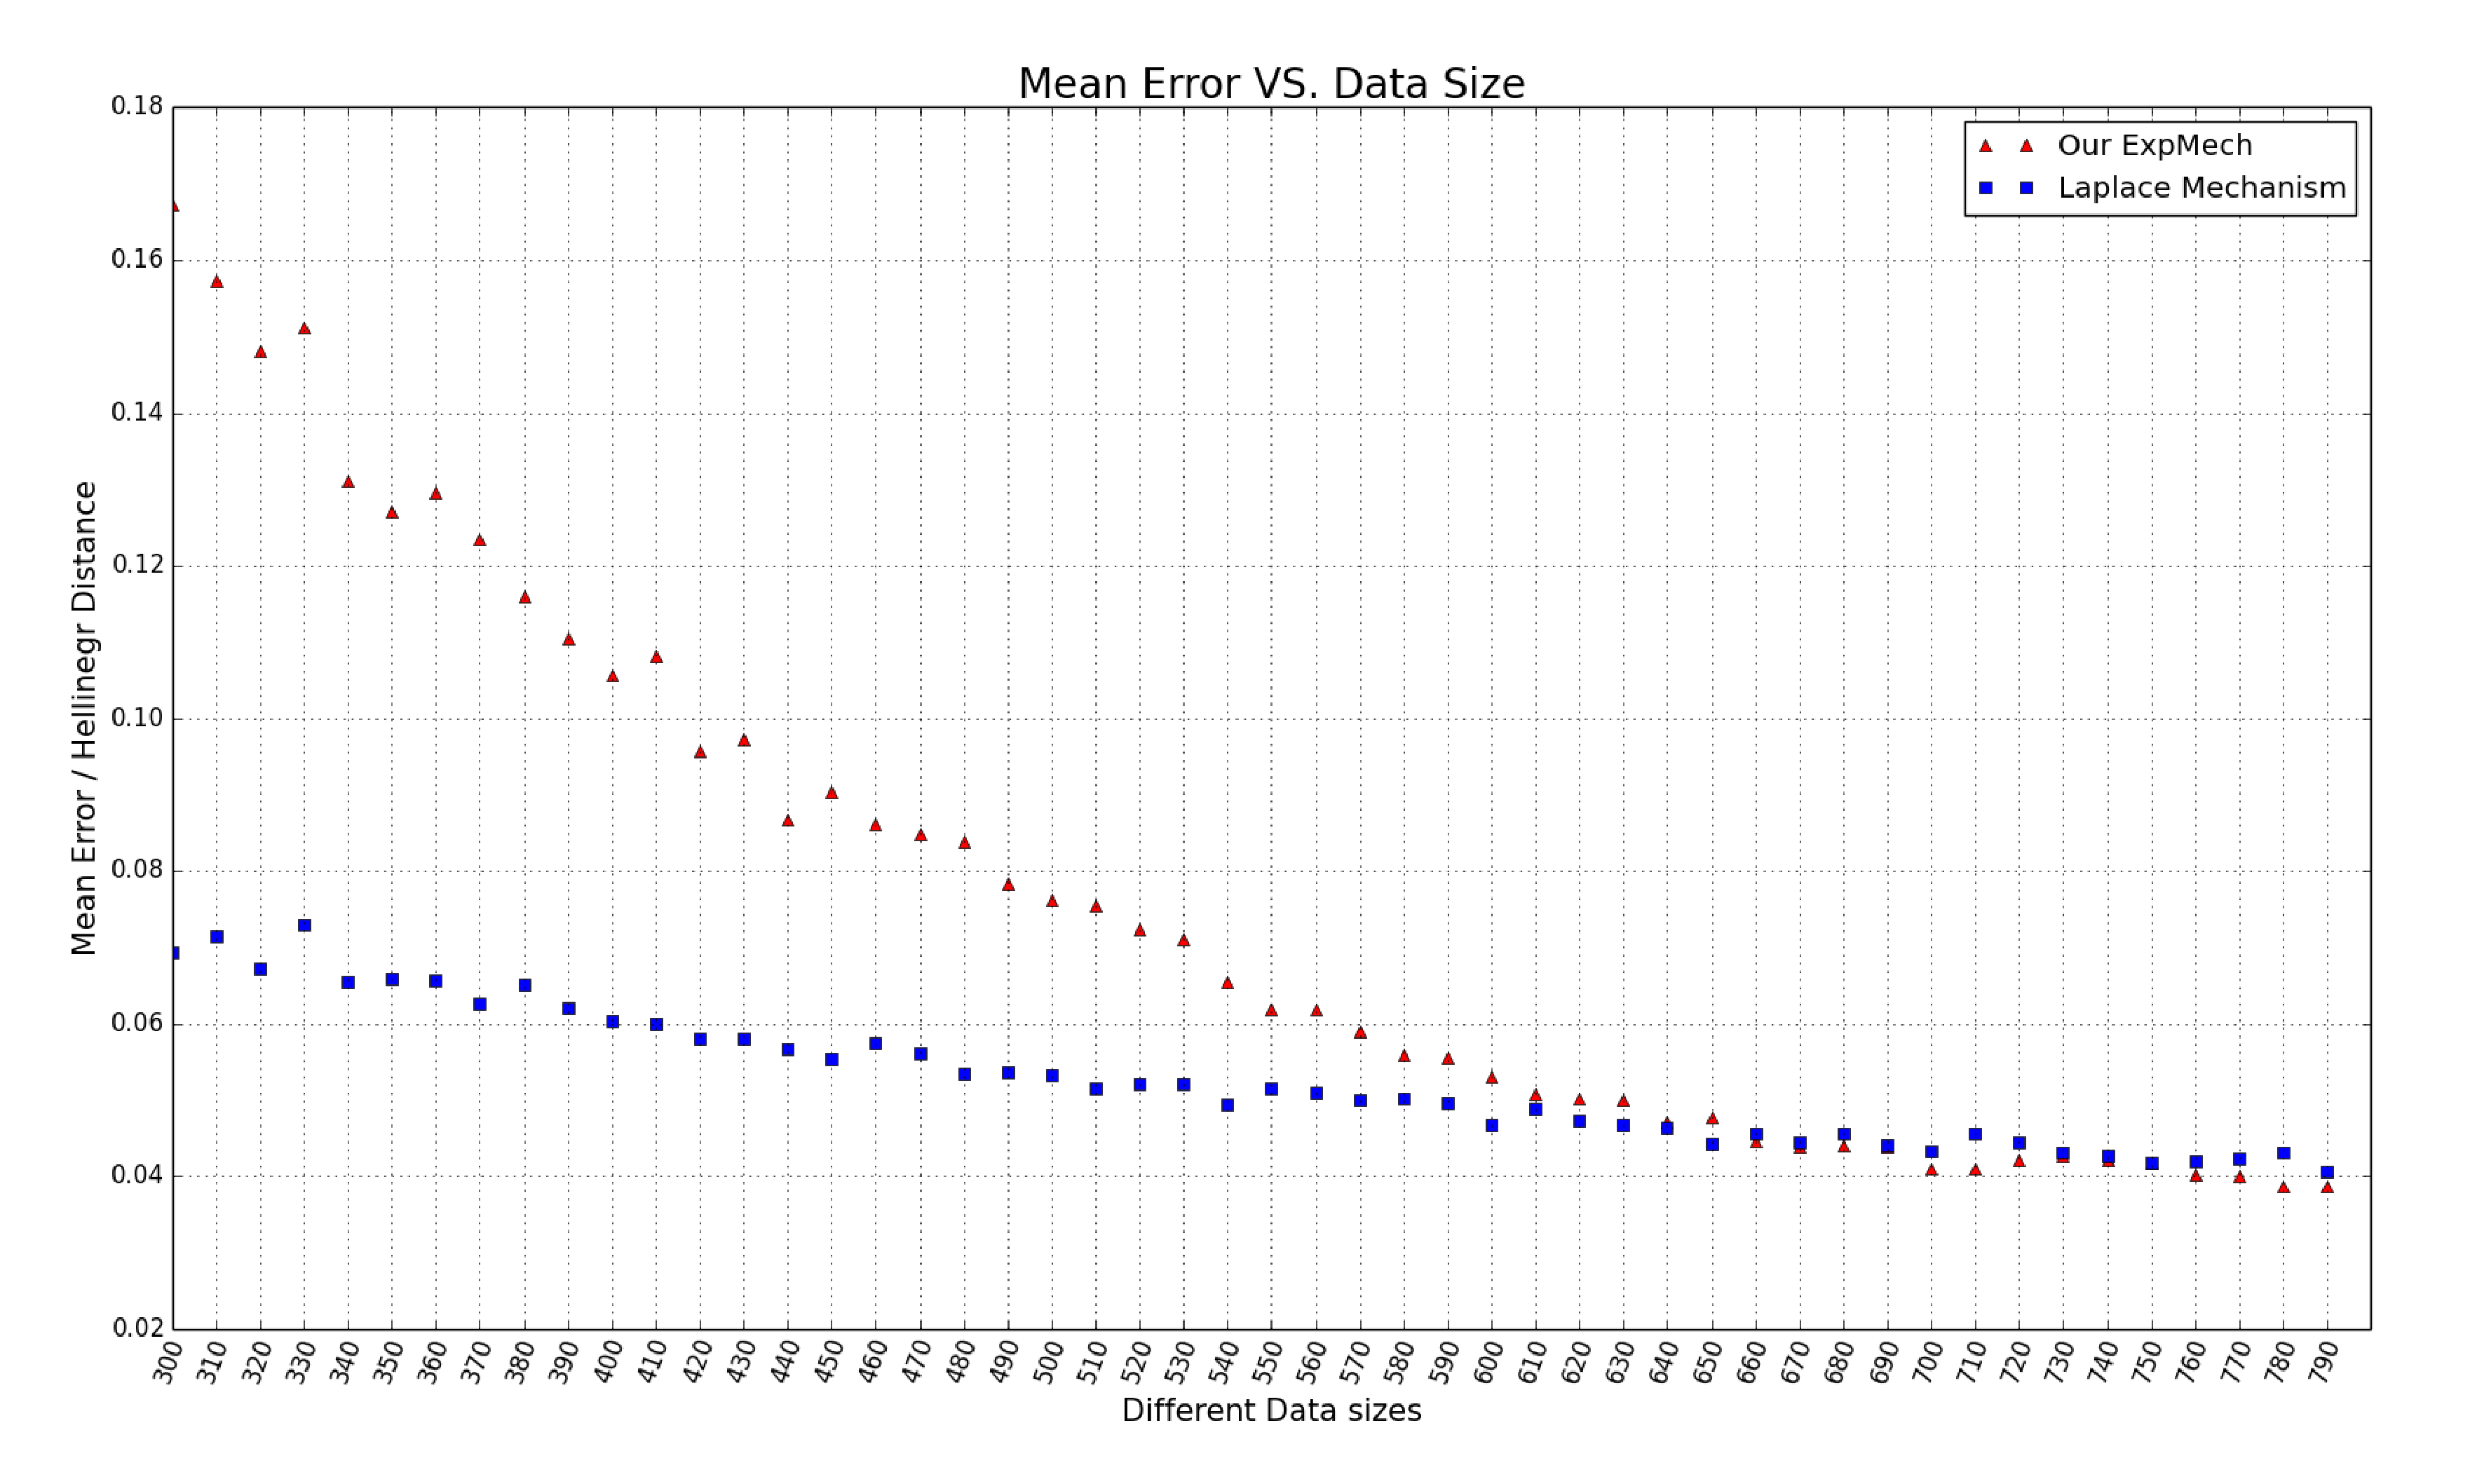
\includegraphics[width=0.45\textwidth]{accuracy_vs_datasize_800.eps}
    \label{subsubsec_vs_datasize1a}
  }
  \subfigure[Data set size from $14000$ to $20000$]{
    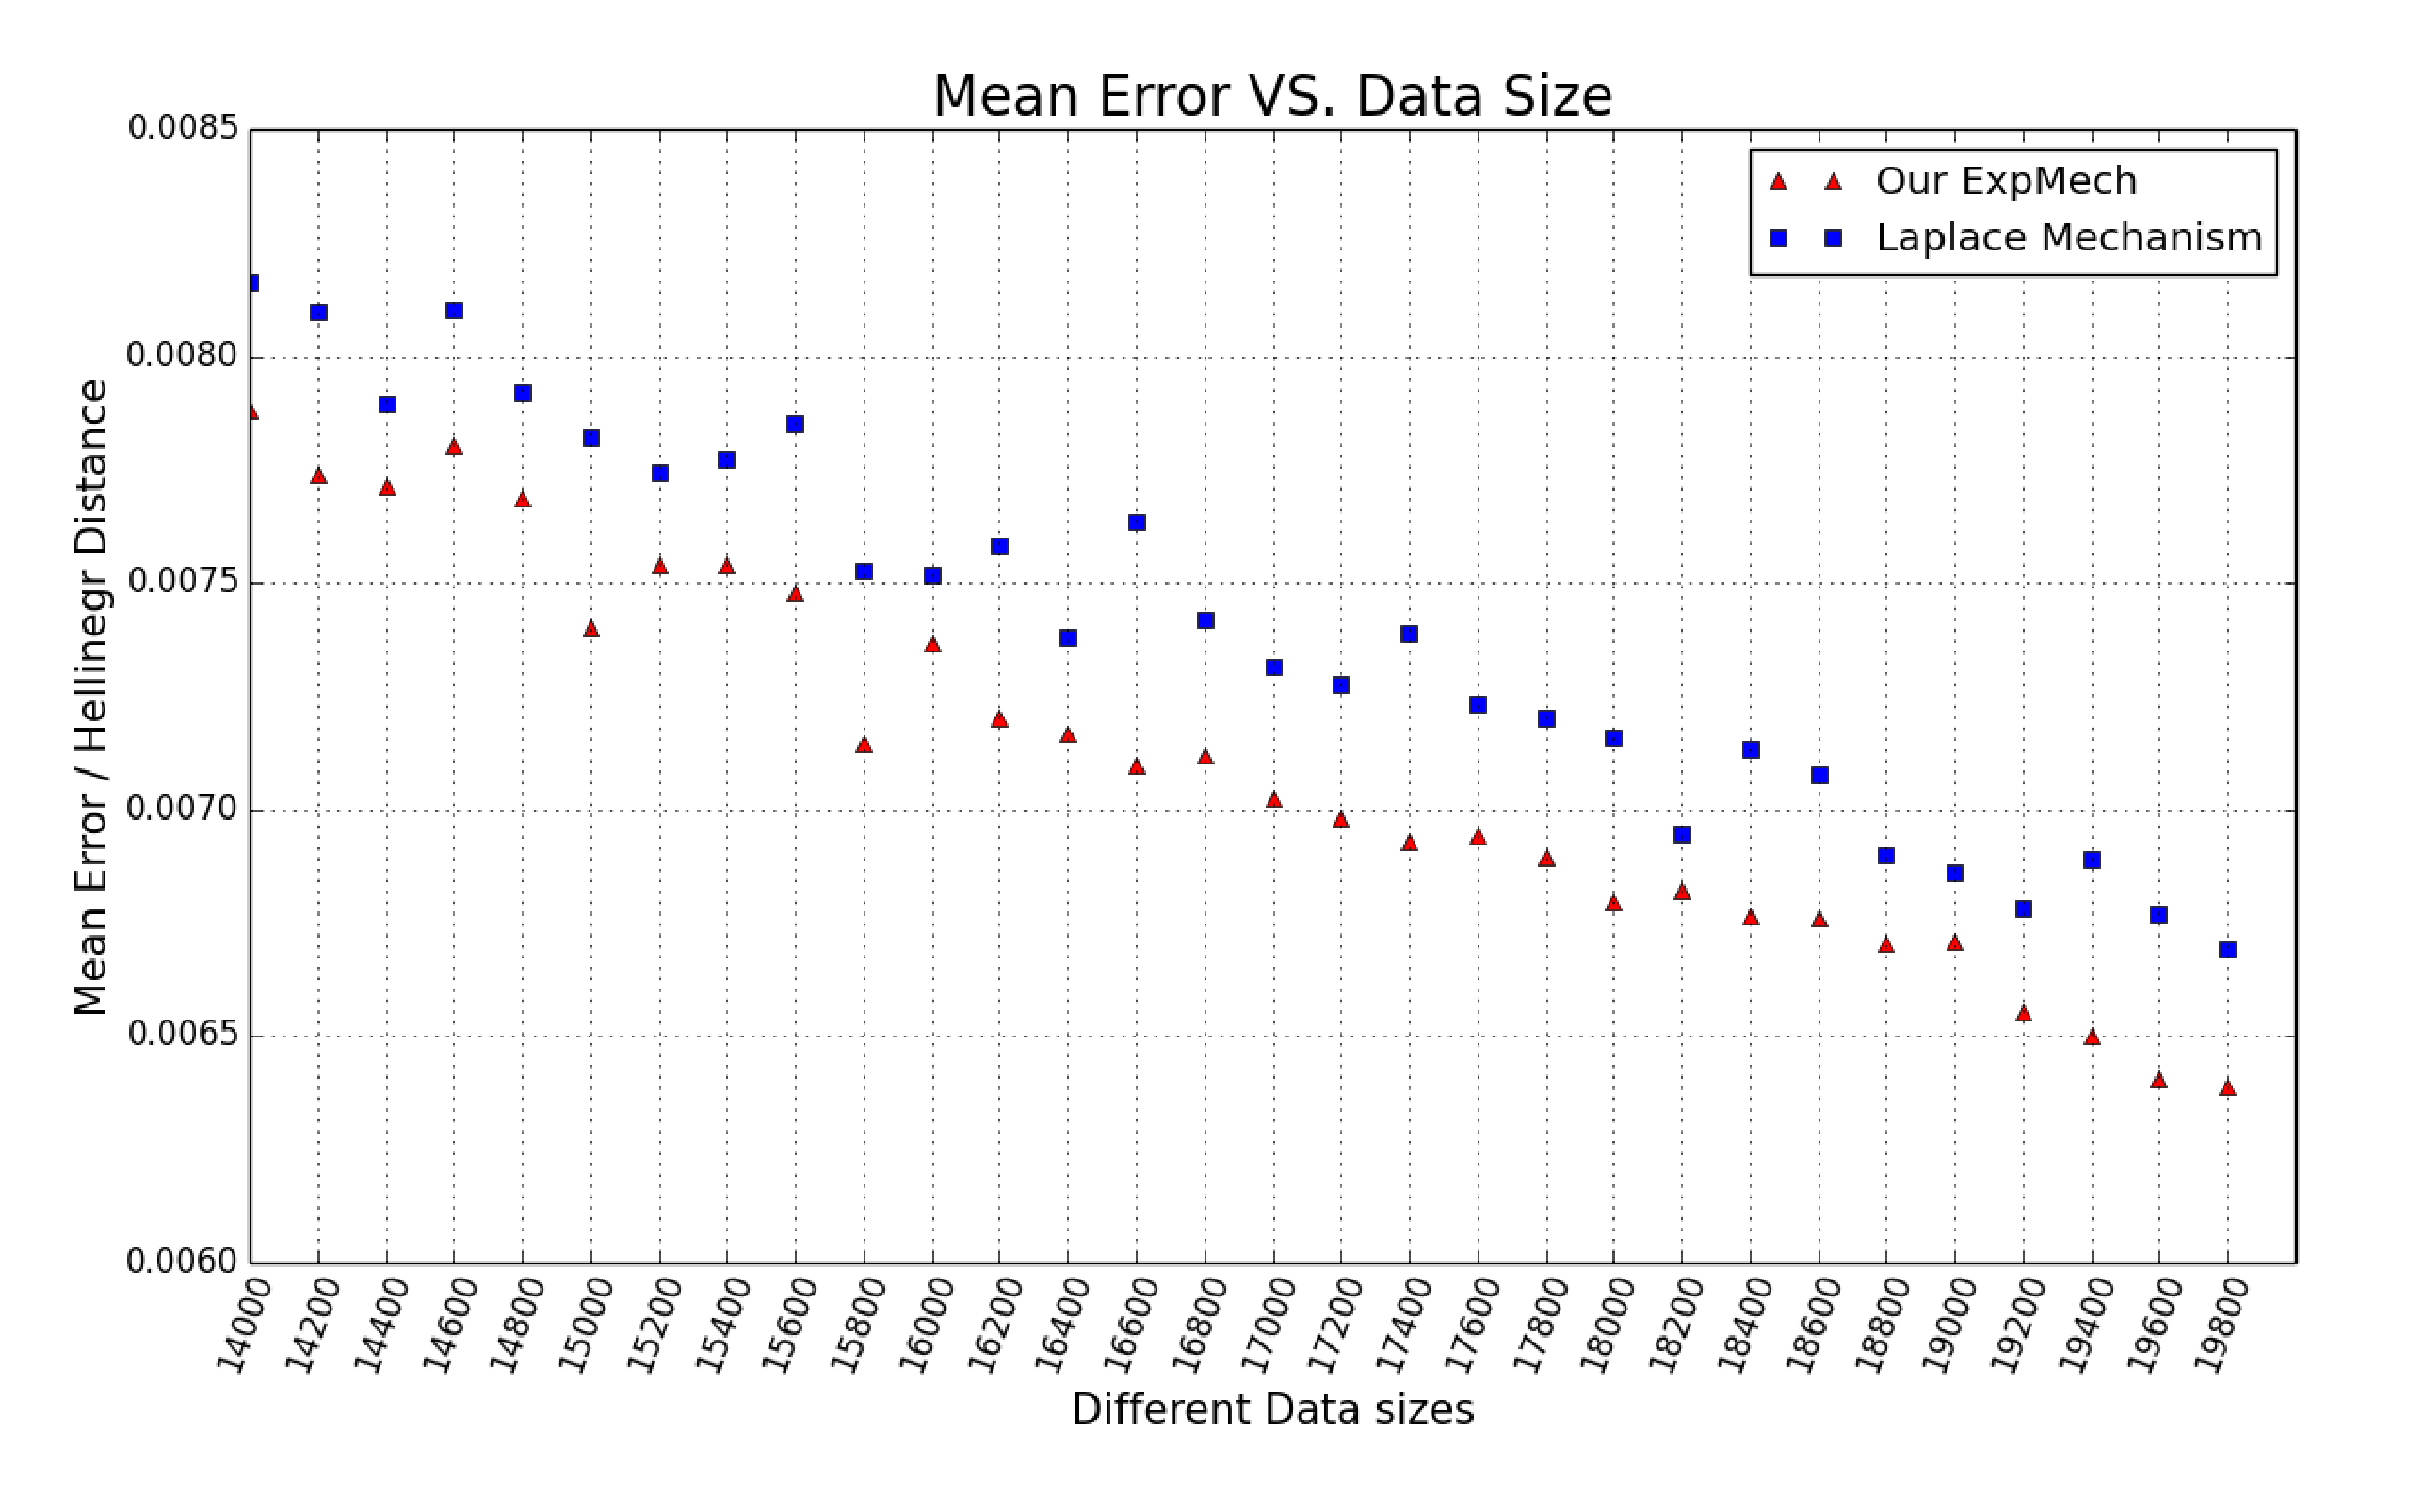
\includegraphics[width=0.45\textwidth]{accuracy_vs_datasize_20000.eps}
  \label{subsubsec_vs_datasize1b}} 
\caption{Increasing data size with fixed prior $\betad(1,1)$. Unbalanced datasets of mean $(0.1,0.9)$ and parameters $\epsilon = 0.8$ and $\delta = 10^{-8}$}
\label{fig_vs_datasize}
\end{center}
\end{figure}

\begin{figure}[ht]
\begin{center}
\centering
  \subfigure[Data set size from $300$ to $800$ ]{
    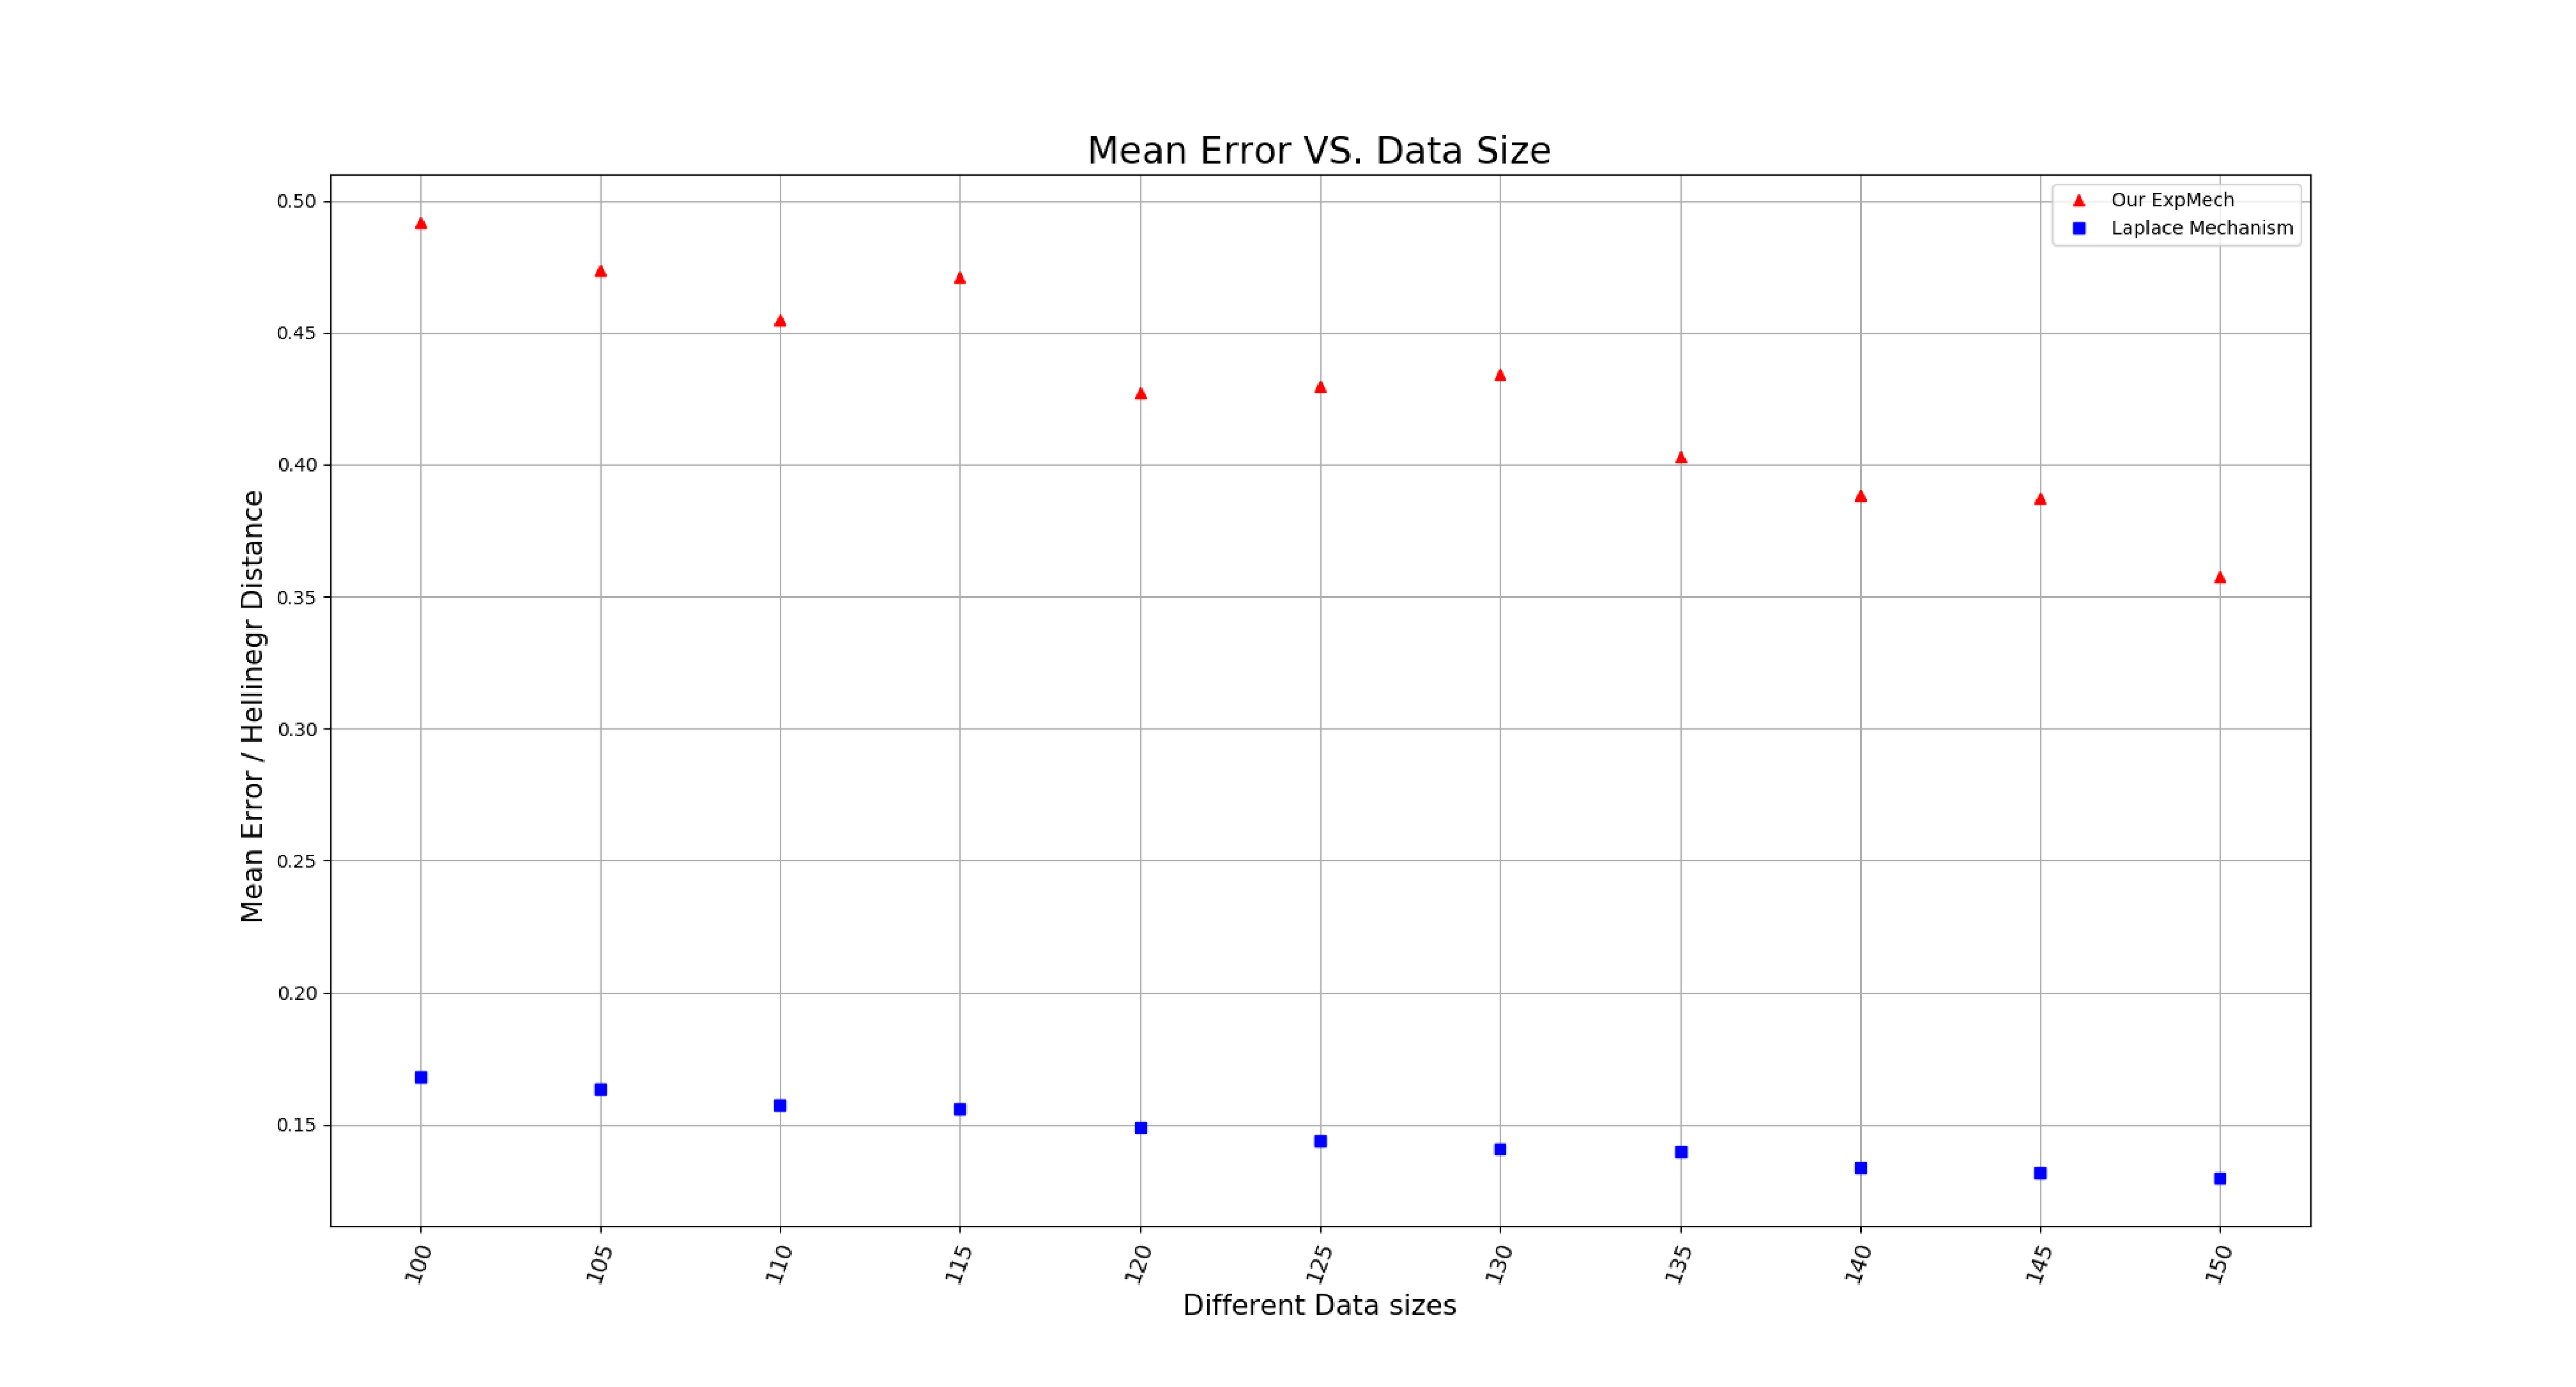
\includegraphics[width=0.45\textwidth]{accuracy_vs_datasize_300_dirichlet.eps}
    \label{subsubsec_vs_datasize1adir}
  }
  \subfigure[Data set size from $14000$ to $20000$]{
     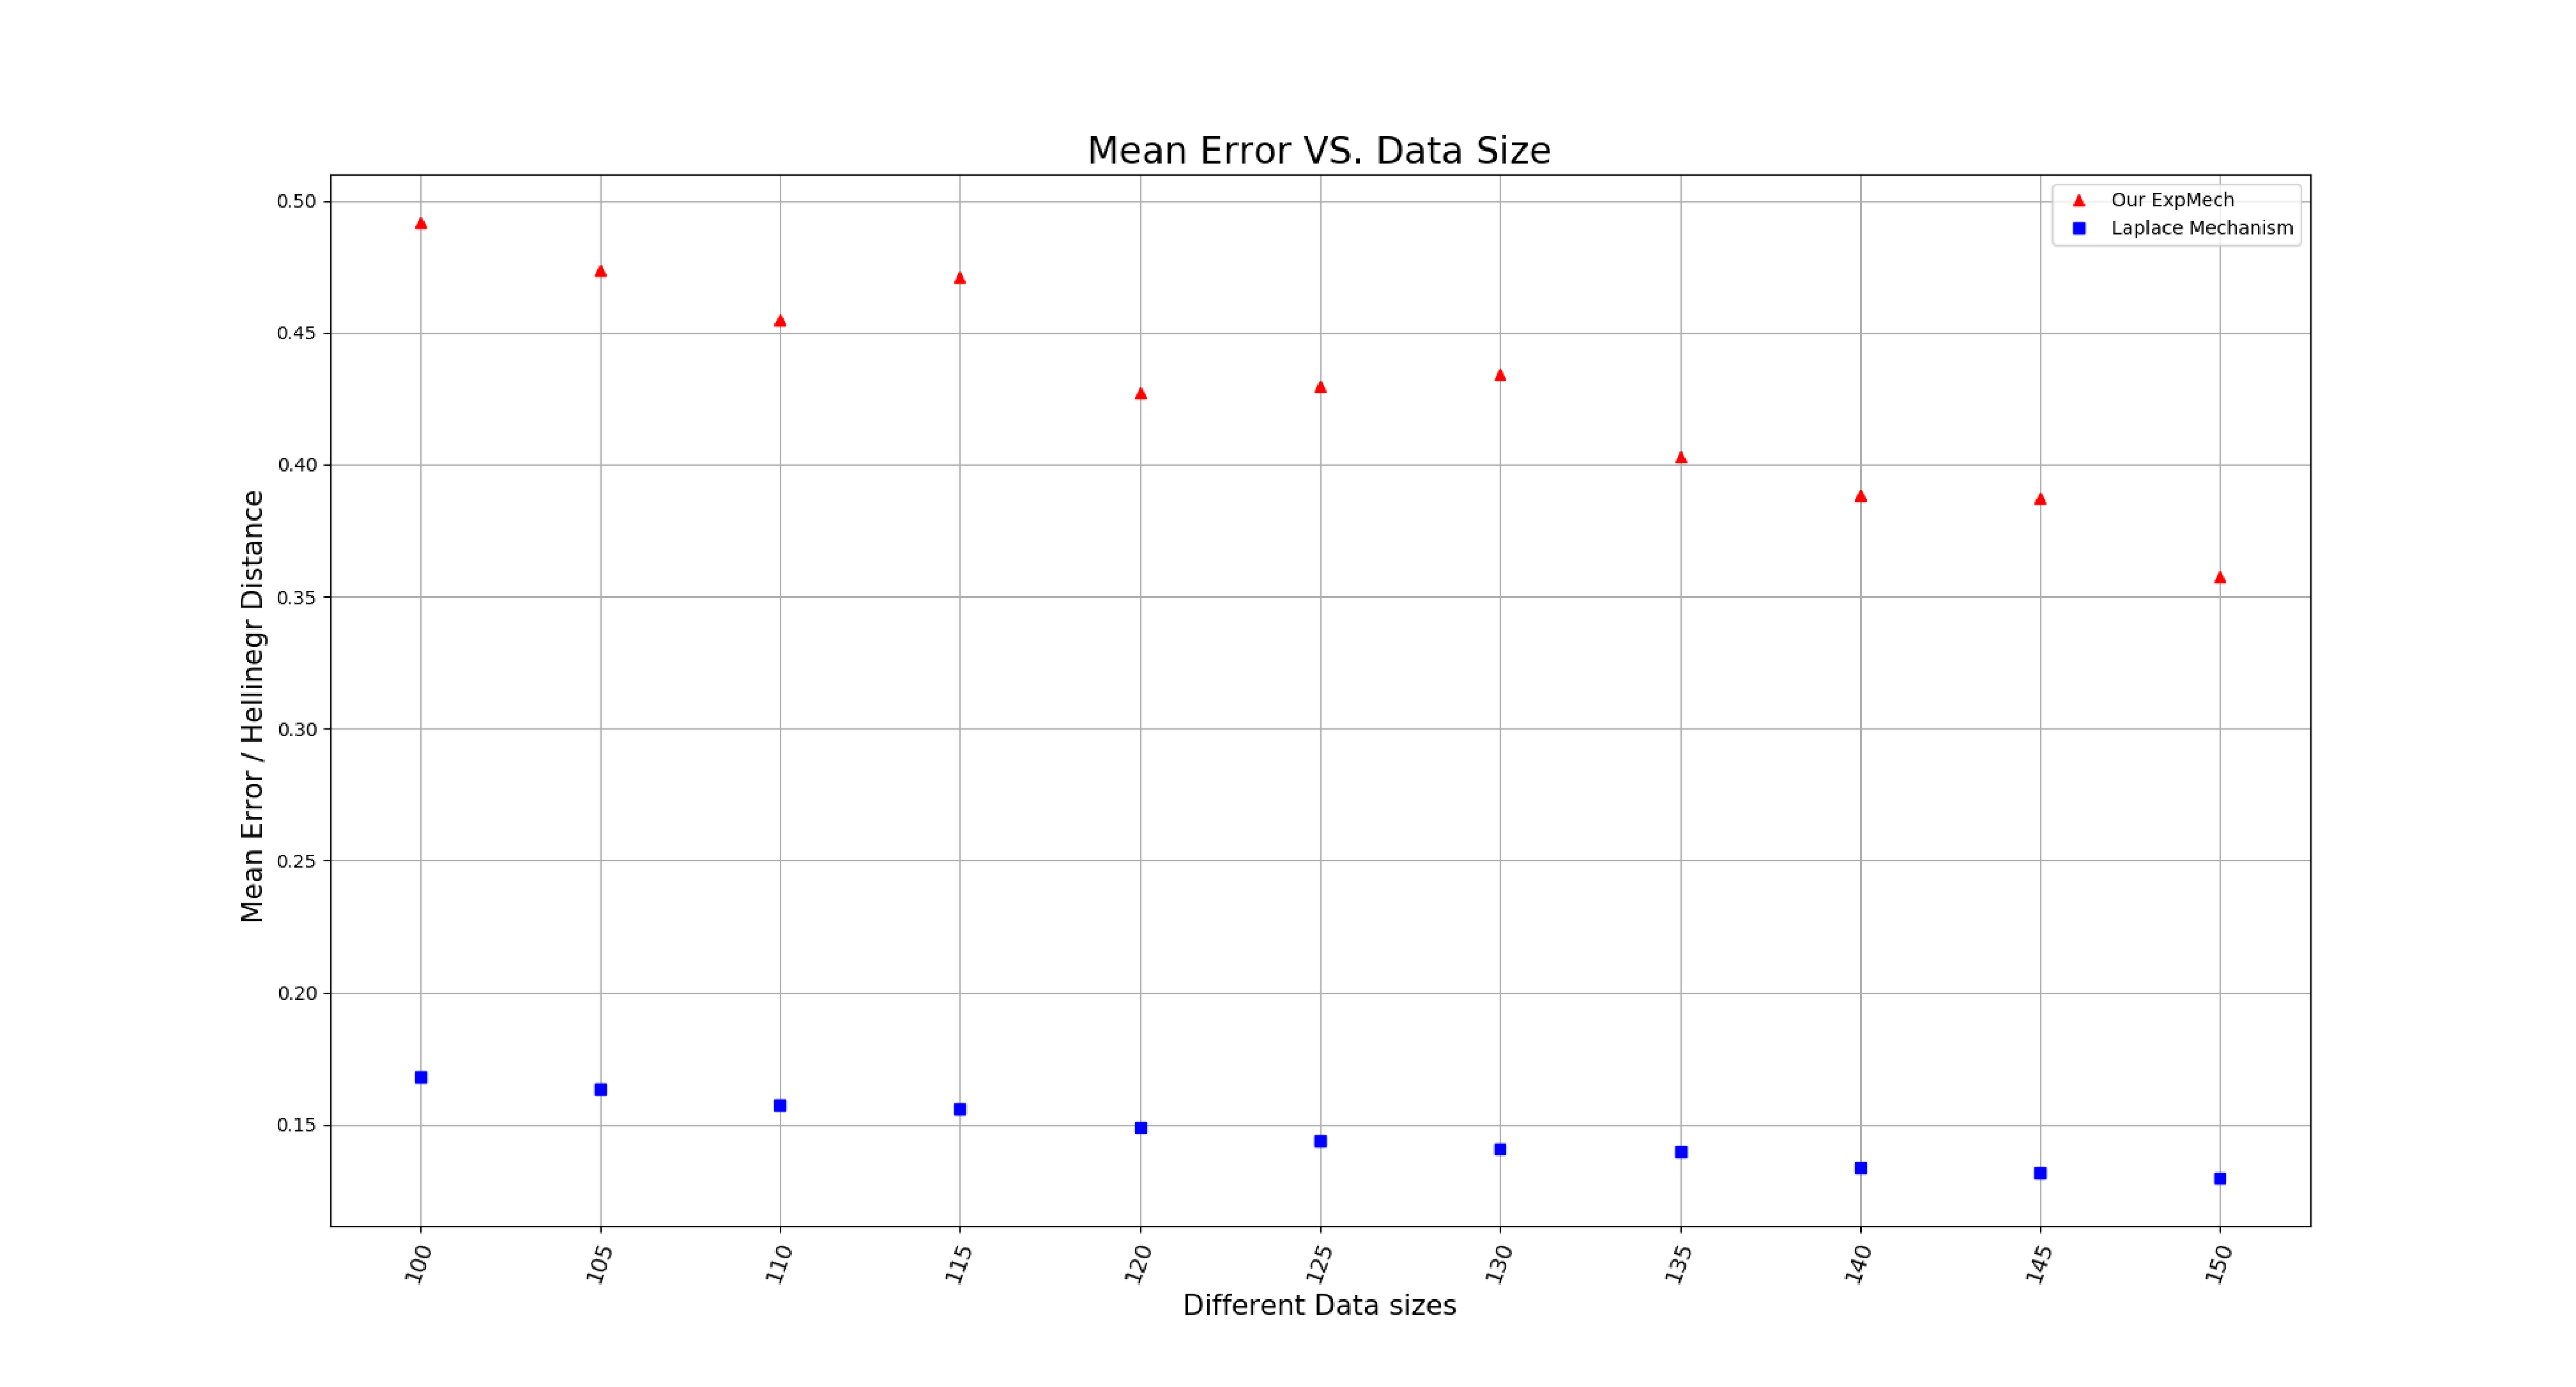
\includegraphics[width=0.45\textwidth]{accuracy_vs_datasize_1k_dirichlet.eps}   
  \label{subsubsec_vs_datasize1bdir}} 
\caption{Increasing data size with fixed $\dirichlet(1,1,1)$ prior distribution, Unbalanced datasets of mean $(0.2,0.3, 0.5)$ and parameters $\epsilon = 0.8$ and $\delta = 10^{-8}$}
\label{fig_vs_datasize_dir}
\end{center}
\end{figure}

In Figures \ref{fig_vs_datasize} and \ref{fig_vs_datasize_dir} we consider \emph{unbalanced} datasets
of observations. This means that in the Beta-Binomial setting (Figure \ref{subsubsec_vs_datasize1a},
and \ref{subsubsec_vs_datasize1b}) the datasets will consist of 10\% 1s and the rest 0s, while for the
Dirichelet-Multinomial (Figure  \ref{subsubsec_vs_datasize1adir} and \ref{subsubsec_vs_datasize1bdir})
the data will be split in the $k=3$ bins with perecentages of: 20\%, 30\% and 50\%.
The results show that when the data size
increases, the average errors of
$\hexpmech$, $\hexpmechd$, and Laplace decrease. For small datasets,
i.e with size less 650 in the case of Beta-Binomial systems,
the Laplace mechanisms outperforms the exponential mechanisms,
but for bigger data sets, that is, bigger than 650, or as in Figure \ref{subsubsec_vs_datasize1b} where
we considered data sets of the order of 15 thousands elements,
the exponential mechanisms outperforms the Laplace mechanism.
Similar experimental tendencies were obtained for the Dirichlet-Multinomial system ( (Figure  \ref{subsubsec_vs_datasize1adir} and \ref{subsubsec_vs_datasize1bdir})),
but we were not able to perform experiments with higher dimensions (4 or more) or, big datasets, e.g. $10^4$ elements, due to
too high run time of the algorithm.



% \paragraph{Increasing dimensions and data size with balanced dataset}
% \label{subsubsec_vs_dimension}
% In Figure \ref{fig_vs_dimension}, in the x-axis are observed data sets
% of different sizes and different dimensions. The plot shows that
% increasing the number of dimensions has a similar pejorative effect on
% $\hexpmech, \hexpmechd$, and the Laplace mechanism. Fixing the number
% of dimensions and increasing the data size shows that the Laplace
% mechanism is more accurate then both $\hexpmech$ and $\hexpmechd$. In
% other words, dimensions have little influence on whether our
% mechanisms will beat the Laplace mechanism.

% \begin{figure}[ht]
% \centering
% 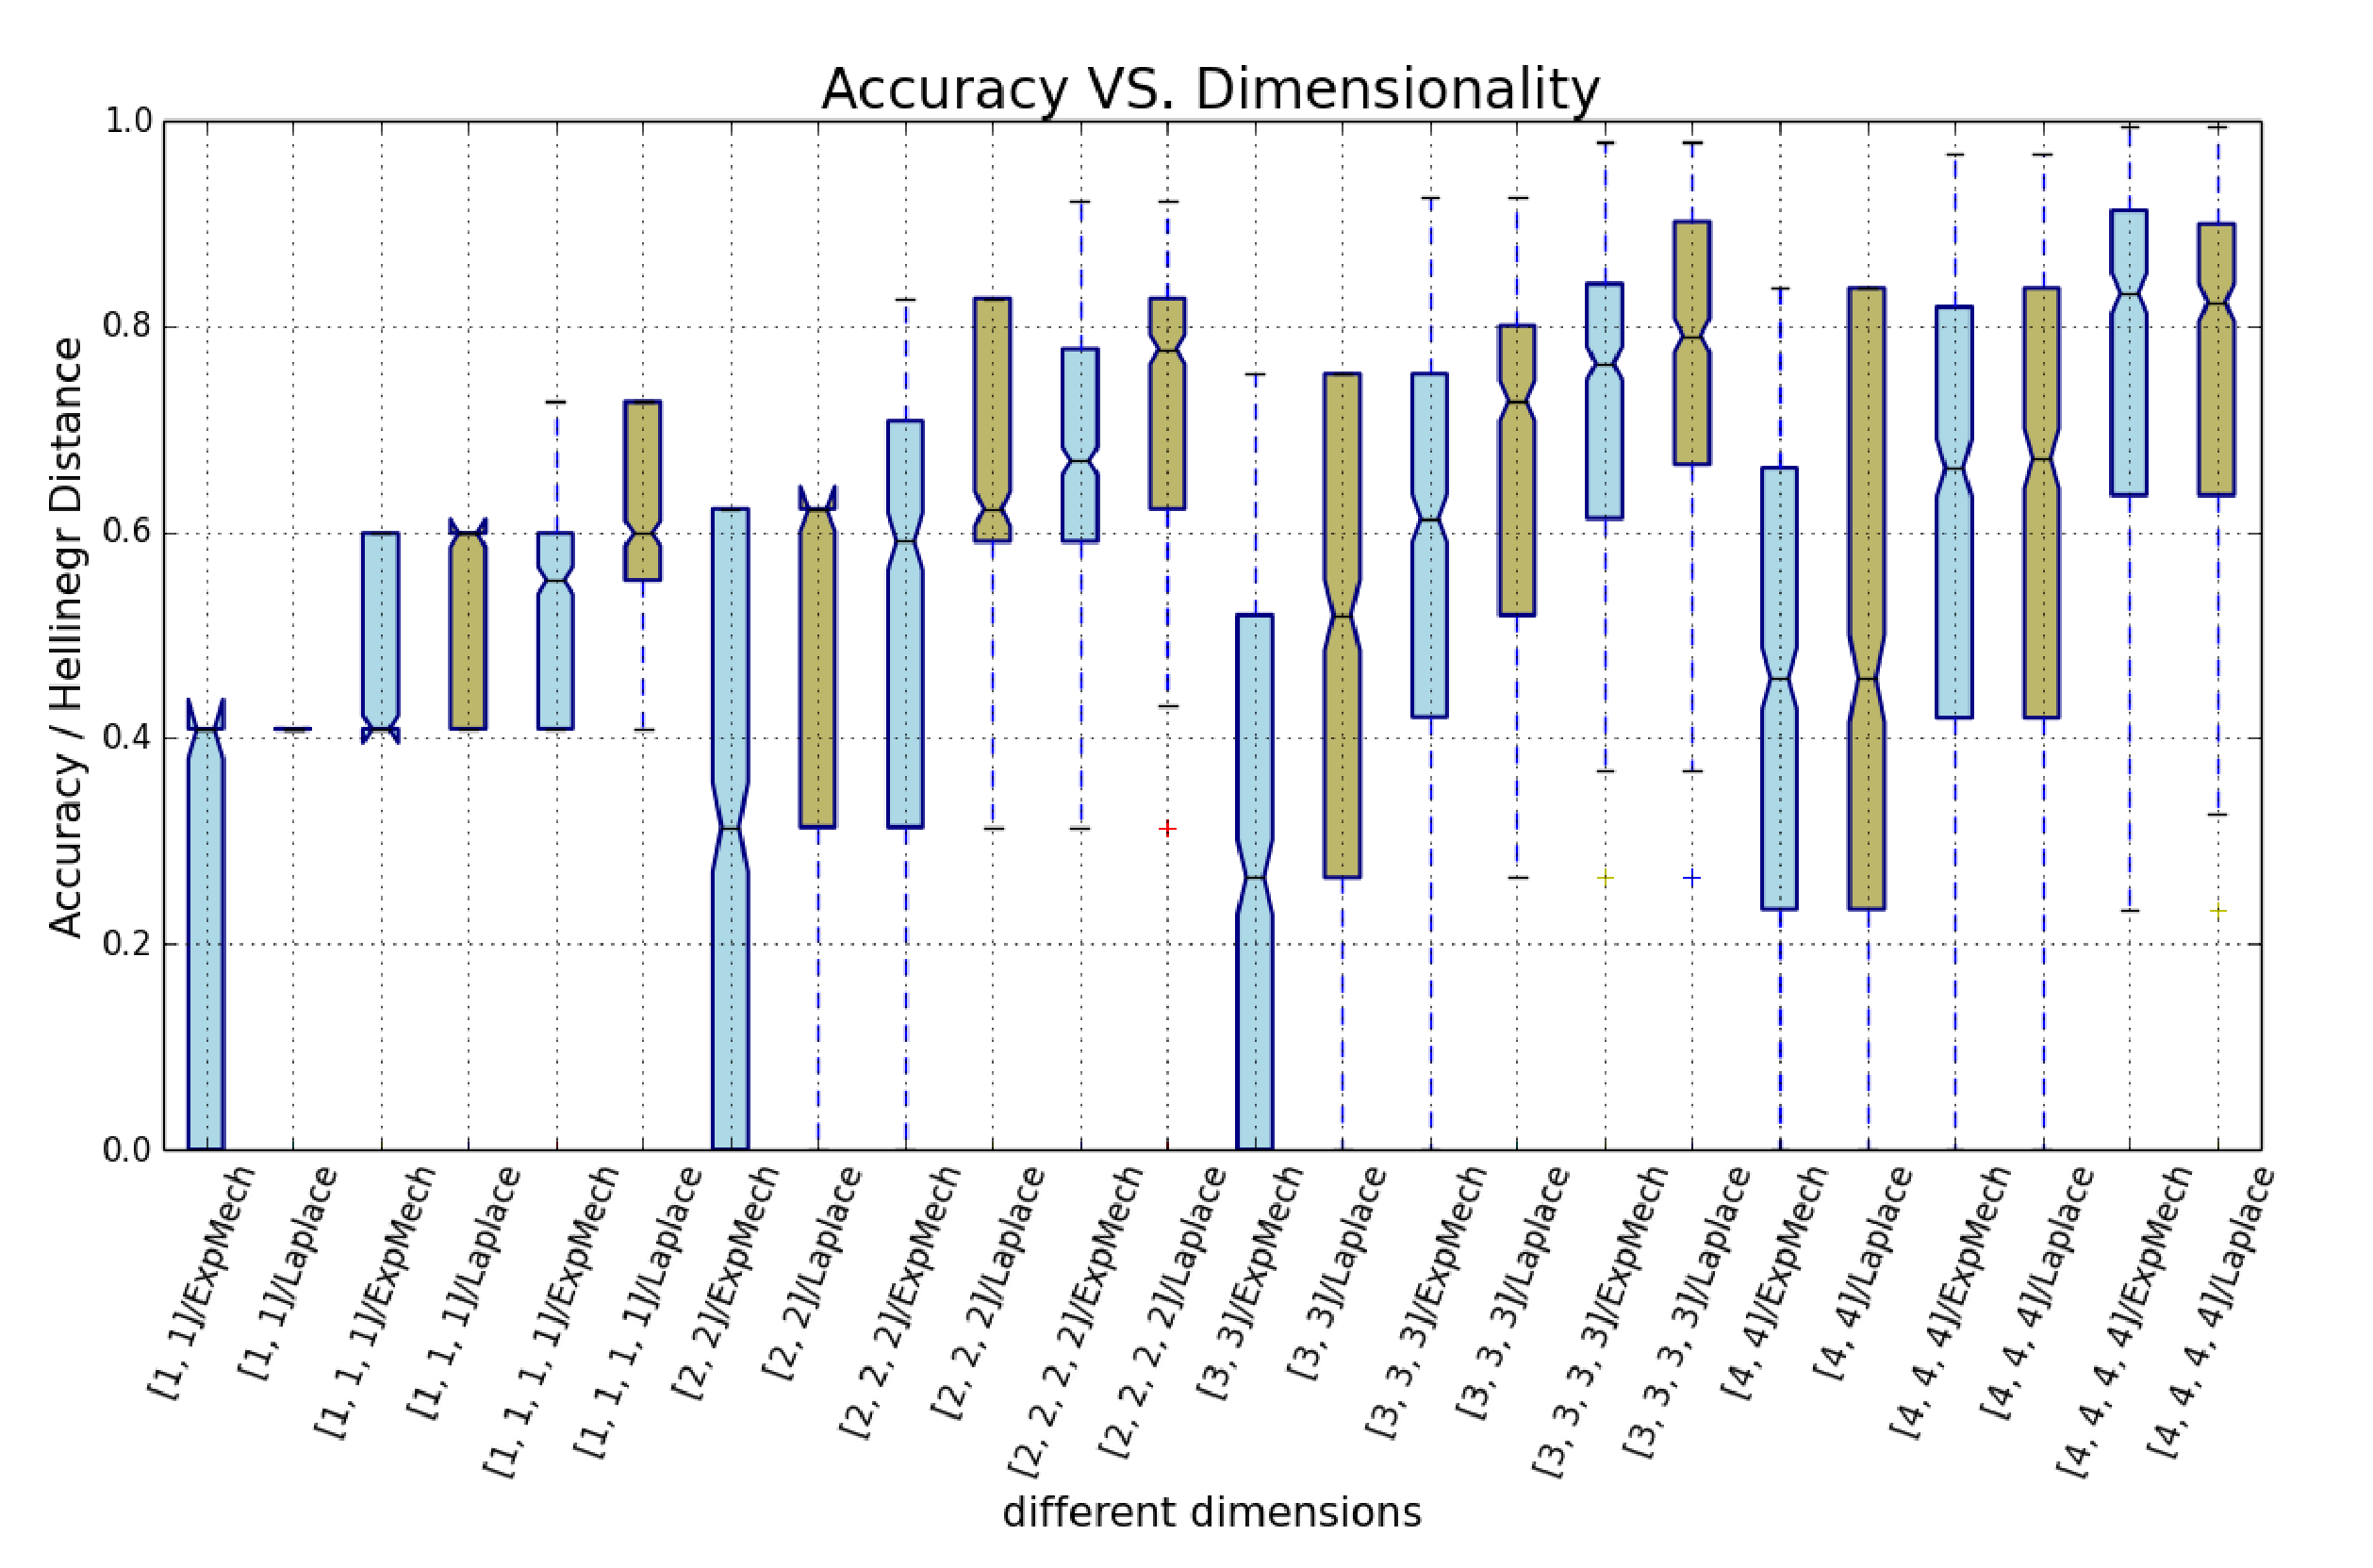
\includegraphics[width=0.45\textwidth]{accuracy_vs_dimension.eps}
% \caption{Increasing dimensions and data size with balanced dataset. Priors have 1s in every dimension.}
% \label{fig_vs_dimension}
% \end{figure}


% \paragraph{Fixed data size and unbalaced datasets}
% \label{subsubsec_vs_variance}
% In Figure \ref{fig_vs_variance}, in the x-axis we considered different
% levels of balance of the datasets. We study this variable only under
% the two-dimensional $\betad$ distribution in order to be more
% concise. The plot shows that $\hexpmech$ accuracy is better than the
% one of Laplace when the dataset is balanced.

% \begin{figure}[ht]
% \centering
% 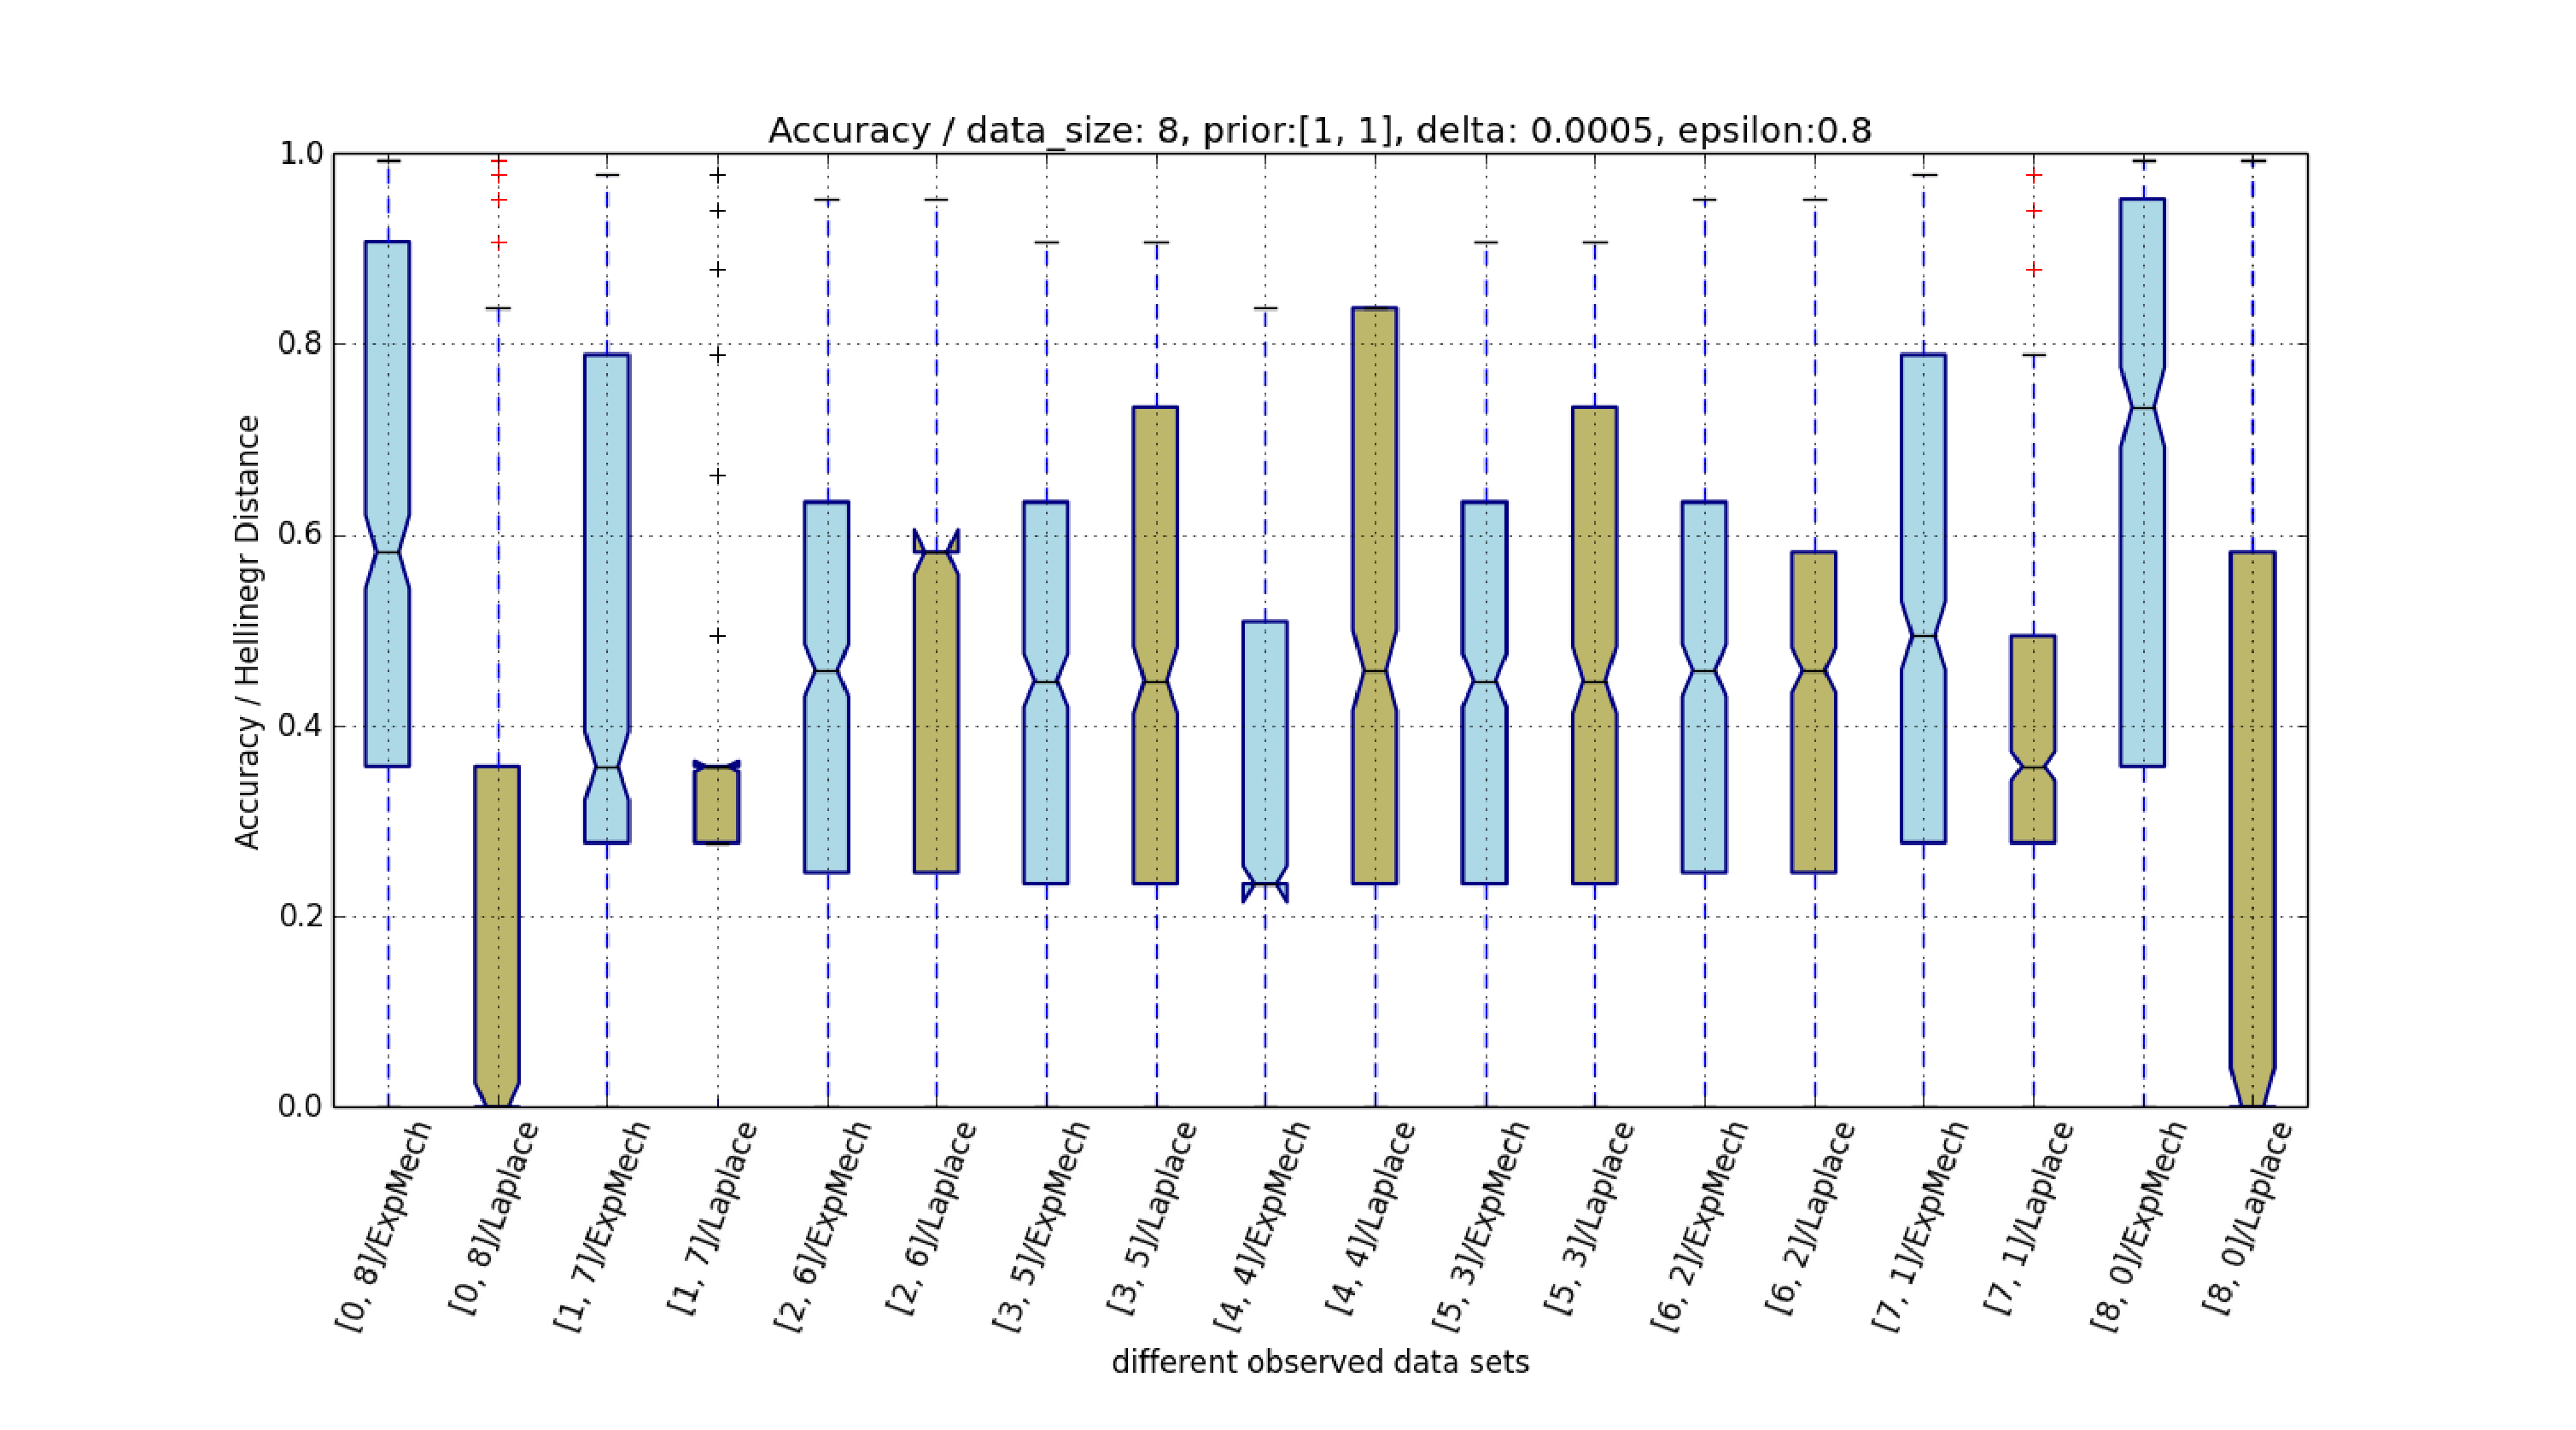
\includegraphics[width=0.45\textwidth]{accuracy_vs_mean_1_1.eps}
% \caption{Unbalanced datasets. Prior distributions have 1s in every dimension.}
% \label{fig_vs_variance}
% \end{figure}




\paragraph{Fixed dataset varying balanced priors}
\label{subsubsec_vs_prior}
In Figure \ref{fig_vs_prior}, we fix the dataset to be $\langle 5,5,5\rangle$.
We also considered balanced priors with increasing values in their dimensions.
The plot shows that in the beginning the Laplace mechanism performs better but
it is outperformed after a while.
\begin{figure}[H]
\centering
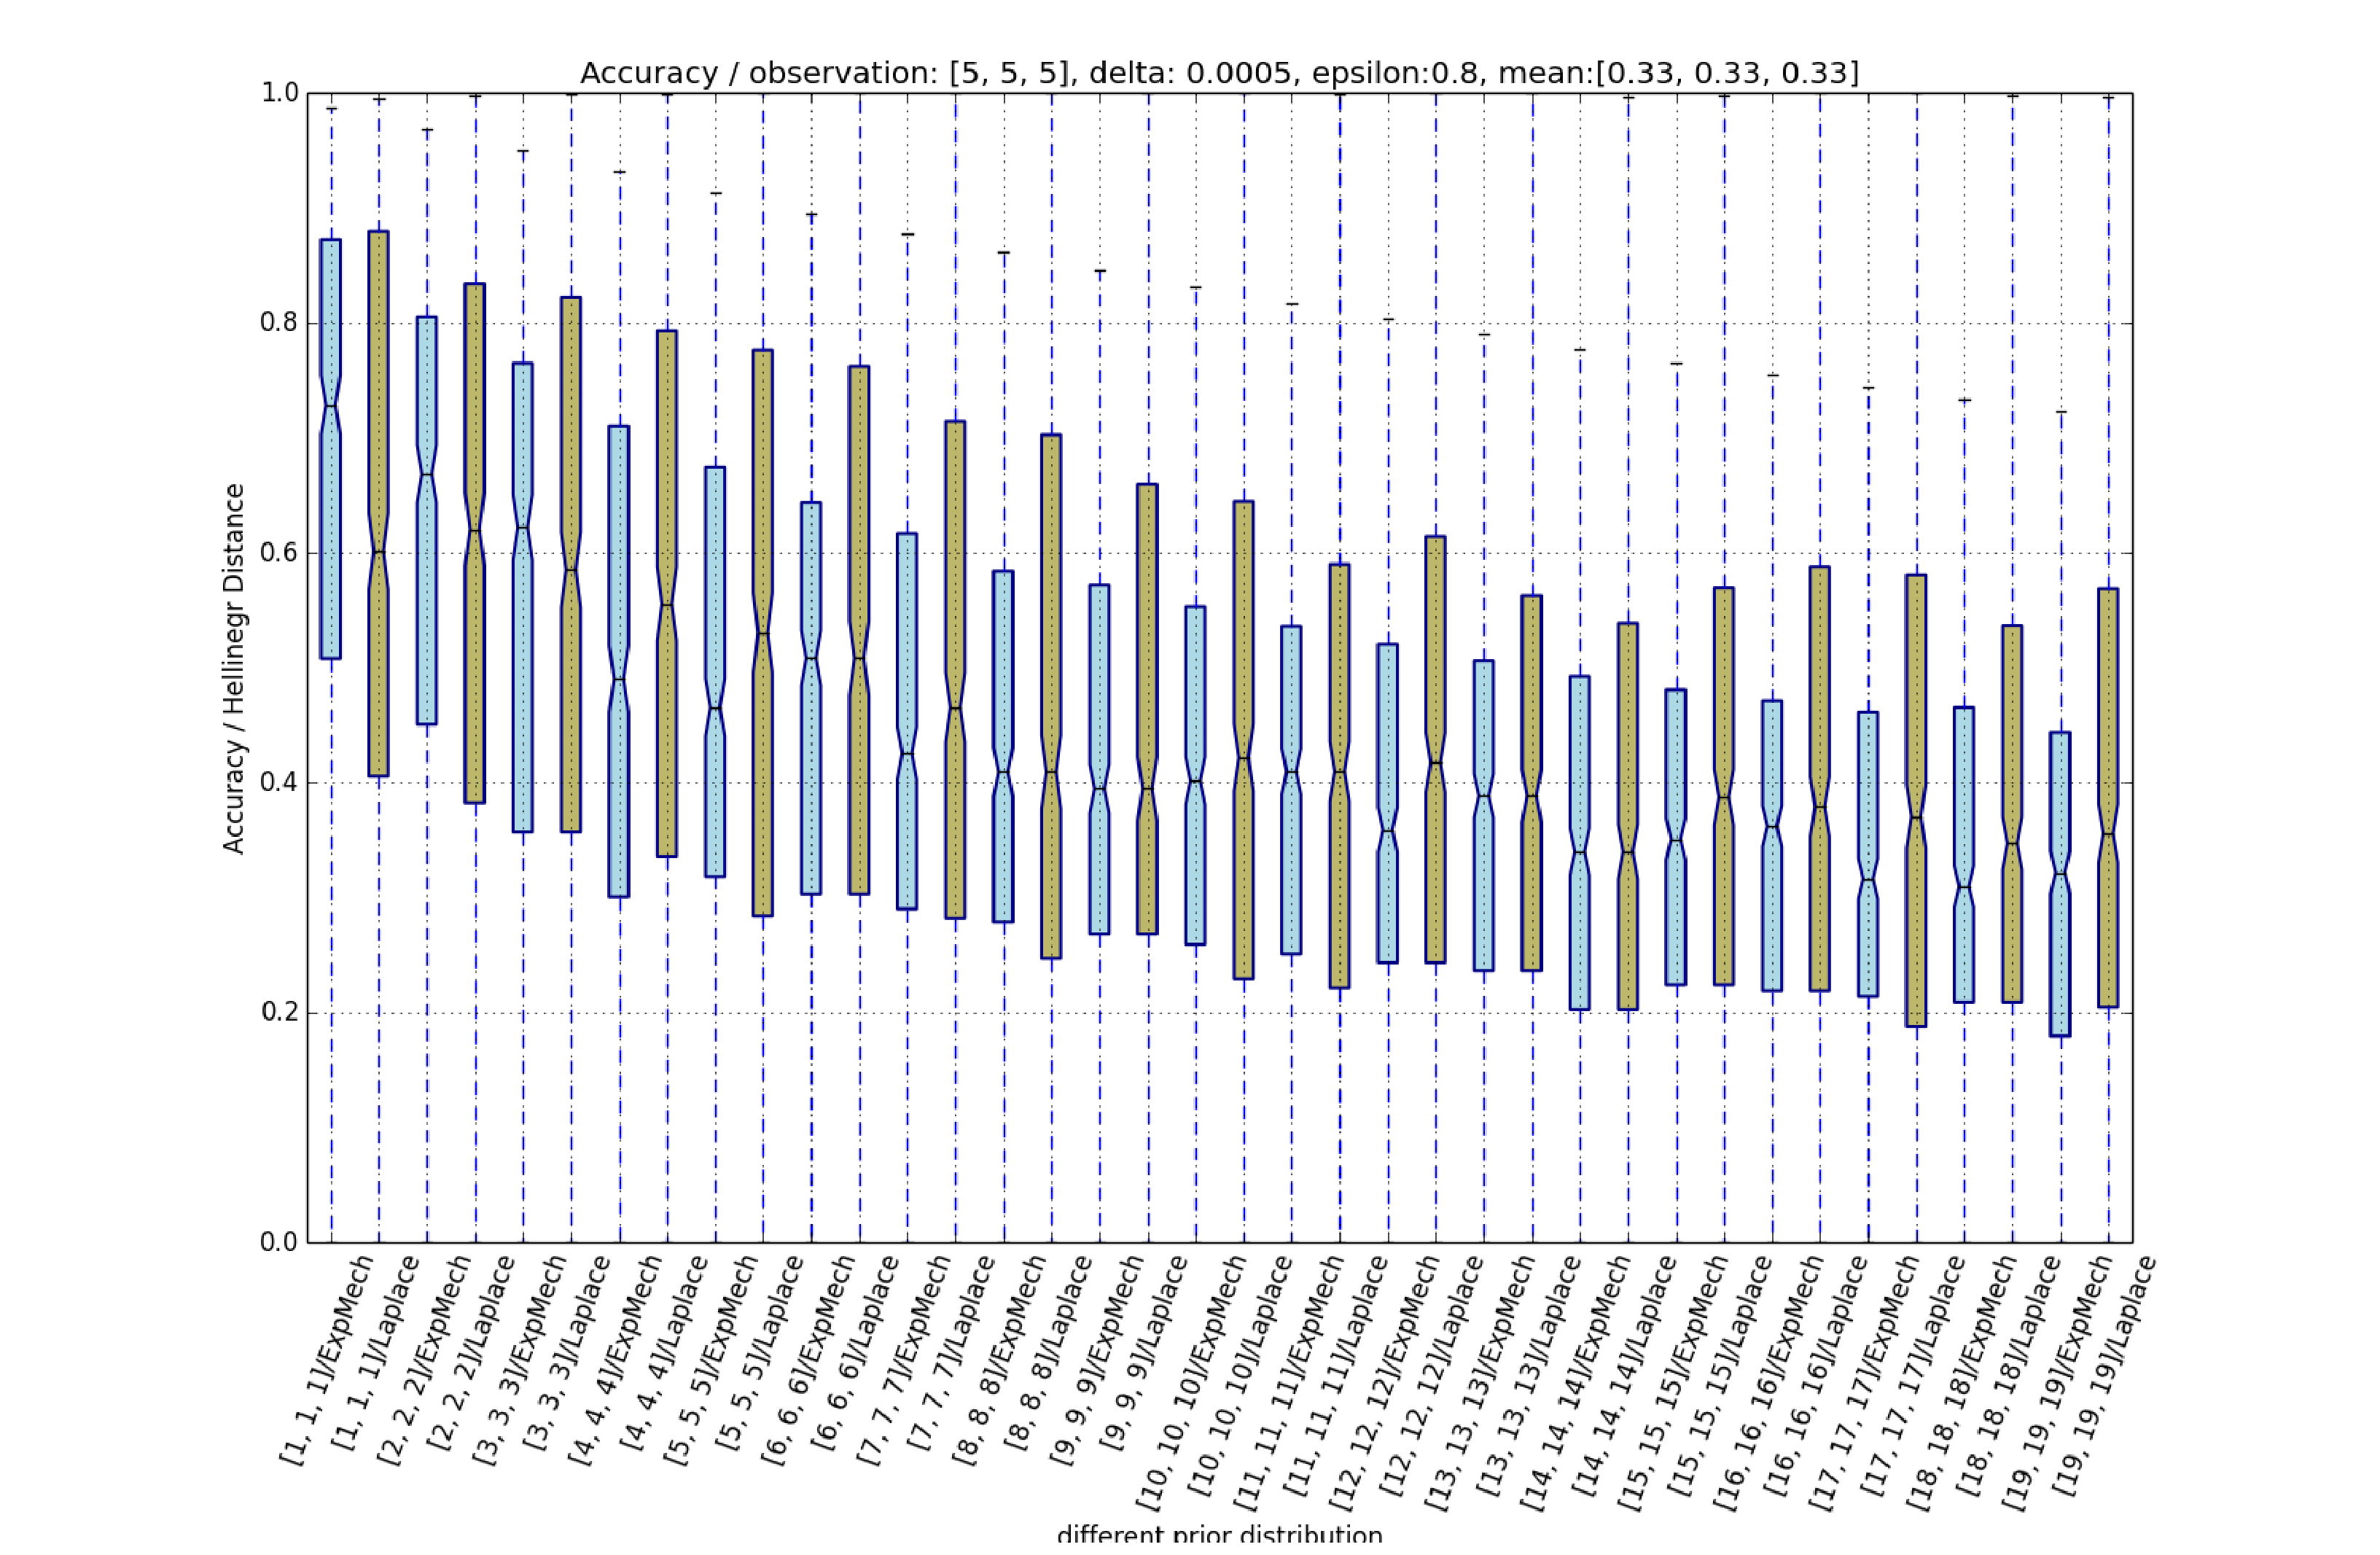
\includegraphics[width=0.45\textwidth]{accuracy_vs_prior_5_5_5.eps}
\caption{Observed data set is: $(5,5,5)$, varying balanced priors}
\label{fig_vs_prior}
\end{figure}





% \subsubsection{Accuracy Evaluation wrt. Prior Distribution and Data Variance}
% \label{subsubsec_vs_prior_variance}

% \begin{figure}[ht]
% \centering
% 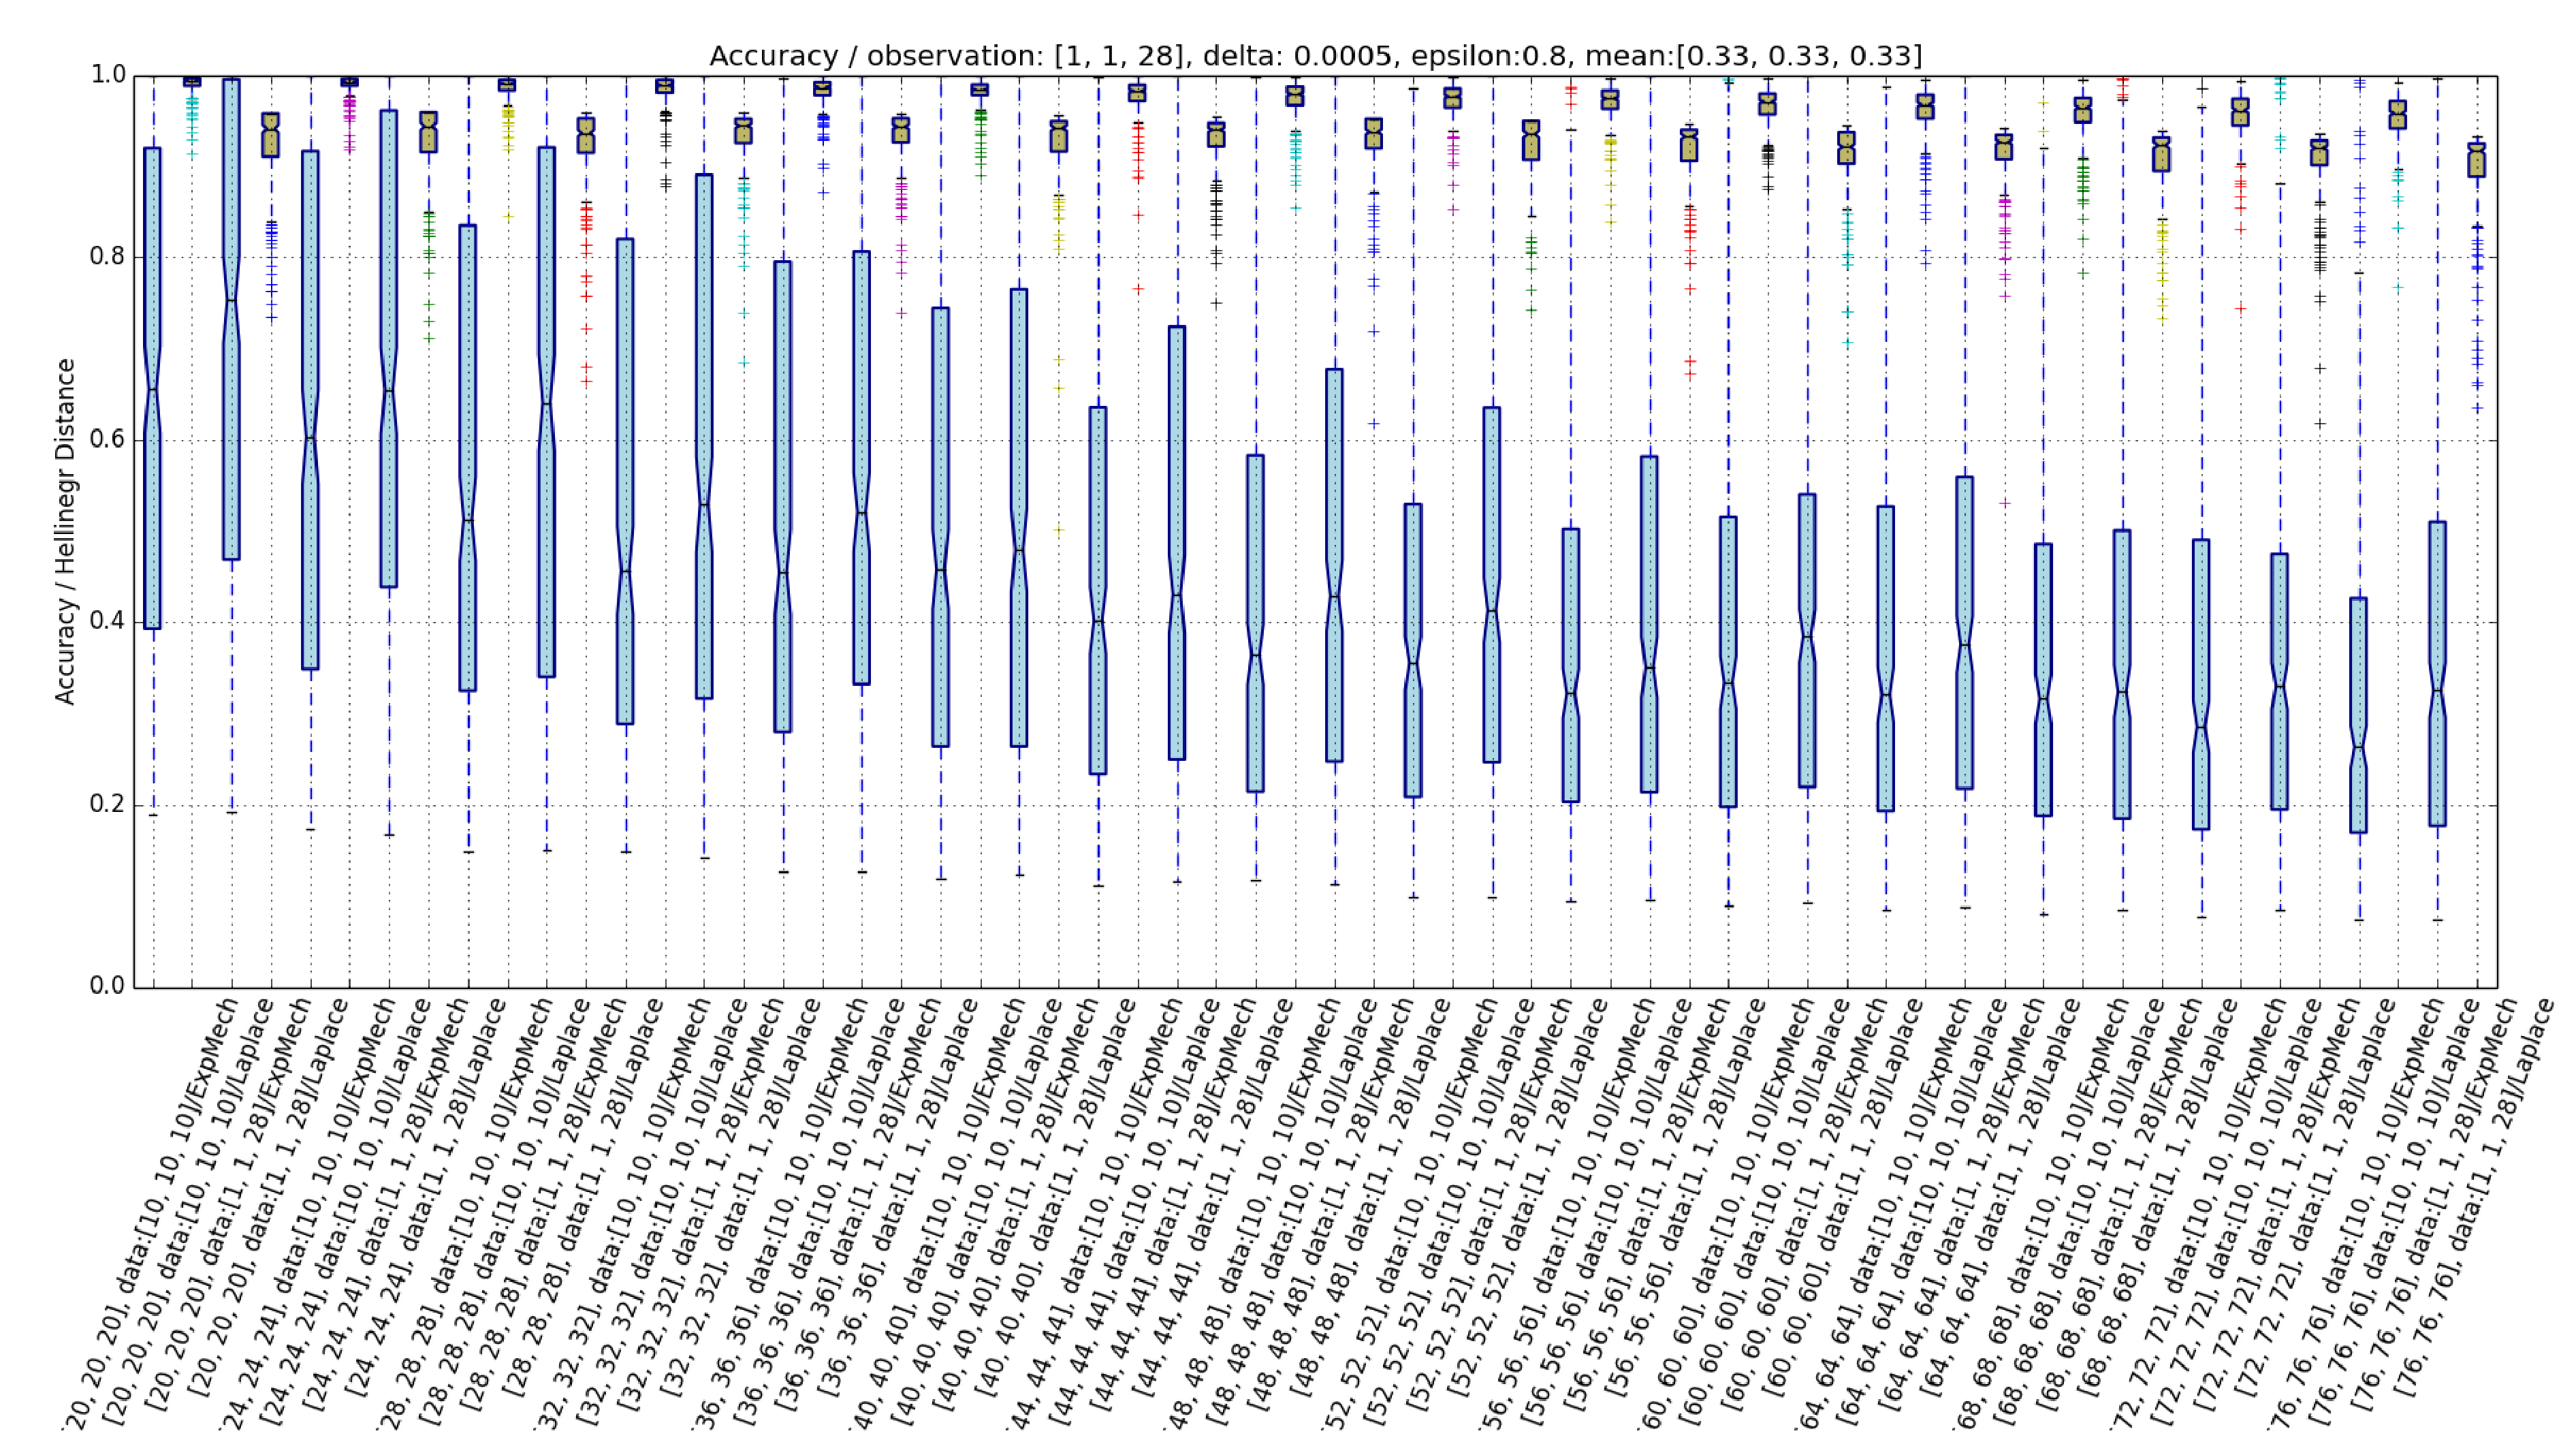
\includegraphics[width=0.45\textwidth]{Accuracy_VS_Prior_mean.eps}
% \caption{Accuracy measurement based on Hellinger distance wrt. different prior distribution and data variances. Settings: $\epsilon = 0.8$ and $\delta = 0.00000001$, observed data sets are $[10,10,10]$ and $[1,1,28]$ and prior distributions are range from $[20,20,20]$ to $[76,76,76]$}
% \label{fig_vs_prior_variance}
% \end{figure}

% Here, we change the prior distribution and data variance in the same time. As shown in Figure  \ref{fig_vs_prior_variance}, our exponential mechanism do better in uniform data set than in edging data set while Laplace mechanism on the contrary. Moreover, our mechanism is improving continuously and significantly as prior distribution increasing while Laplace mechanism isn't.


\section{Conclusions and Future Works}
From what we have seen in the previous sections we can obtain some preliminary conclusions. That is, the probabiliy measure approach outperforms the $\ell_1$-norm approach in the following cases: 
\begin{enumerate}
  \item When the data size is small, data is balanced and priors parameters increase
  \item When the data size is large
\end{enumerate}

These results although very motivating, are still not enough for real world applications. Hence, we will continue our work in the follwoing directions:
\begin{enumerate}
  \item  For now, we just have a intuitive idea on the accuracy
behavior of our mechanisms, and not a precise formula or bound on
it. When do our mechanisms perform better than the baseline mechanism
and when they don't? How much influence will elements in Section
\ref{sec_experiment} have on the accuracy? Are there any other
important factors we missed? These are all questions w.r.t. the
accuracy that we are going to explore next, and in a more principled
and formal way.
\item  Theorem \ref{thm:privacy} provides an upper bound on the
privacy loss for $\hexpmech$ and $\hexpmechd$ but not necessarily a
tight one. Indeed, experiments have shown that the actual privacy loss
in the experiments can be smaller than $\epsilon$. This means that we
could improve accuracy, by adding less noise -- that is noise
proportional to a higher value of $\epsilon$-- but still achieve
$(\epsilon, \delta)$-dp.
\item The choice of the Hellinger distance might seem quite
ad-hoc. Hence, it is worth exploring other distances over
distributions. An interesting class of probability metrics is the
family of $f$-divergences \cite{CIT-004}.
\end{enumerate}



\bibliographystyle{ACM-Reference-Format}
\bibliography{bayesian.bib}

\end{document}